%==================================================================
% PROPOSAL PENELITIAN METODOPEN — DESAIN KUNCI (final)
% Sensitivitas produk elevasi global terhadap flood susceptibility
% mapping berbasis Random Forest terkontrol (SRTM vs GLO-30 vs AW3D30)
% Struktur: BAB I 1.1-1.6 | BAB II 2.1-2.10 | BAB III 3.1-3.11 | BAB IV hasil pendahuluan (kernel v24; audit v22 dua skala; bridging v23)
%==================================================================

\documentclass[12pt]{article}

\usepackage[utf8]{inputenc}
\usepackage[T1]{fontenc}
\usepackage{amsmath}
\usepackage{lmodern}% newtx (Times) Type1 tidak tersedia di MiKTeX ini (hanya OTF); fallback lmodern
\usepackage{graphicx}
\usepackage[a4paper,left=4cm,right=3cm,top=3cm,bottom=3cm]{geometry}
% microtype dimatikan: konflik newtx + MiKTeX bitmap fonts
\usepackage{setspace}
\usepackage{enumitem}% tocloft dihapus: tidak cocok dengan kernel LaTeX ini (tagging socket belum didukung)
\usepackage{booktabs}
\usepackage{array}
\usepackage{tabularx}
\usepackage{adjustbox}
\usepackage{float}
\usepackage{caption}
\renewcommand{\figurename}{Gambar}
\renewcommand{\tablename}{Tabel}
\usepackage{placeins}
\usepackage{csquotes}
\usepackage{titlesec}
\usepackage{tikz}
\usetikzlibrary{arrows.meta,positioning,calc}
\usepackage[
backend=biber,
style=numeric-comp,
sorting=none,
giveninits=true,
doi=true,
url=true
]{biblatex}
\addbibresource{references.bib}
\usepackage{fancyhdr}
\usepackage[hidelinks]{hyperref}

%==================================================================
% PENGATURAN BAHASA, NOMOR, DAN JUDUL BAB
%==================================================================

\renewcommand{\contentsname}{Daftar Isi}
\renewcommand{\refname}{Daftar Pustaka}
% numwidth default cukup

% Nomor bab gaya proposal Indonesia: BAB I, II, ... tetapi subbab 1.1, 1.2, ...
\renewcommand{\thesection}{\Roman{section}}
\renewcommand{\thesubsection}{\arabic{section}.\arabic{subsection}}
\renewcommand{\thetable}{\arabic{table}}
\renewcommand{\thefigure}{\arabic{figure}}

% Judul bab terpusat: "BAB I  PENDAHULUAN"
\titleformat{\section}[display]
  {\centering\bfseries\large}
  {BAB \thesection}
  {0.3ex}
  {\MakeUppercase}
\titlespacing*{\section}{0pt}{0pt}{2.2ex}

\titleformat{\subsection}
  {\bfseries\normalsize}
  {\thesubsection}
  {0.75em}
  {}
\titlespacing*{\subsection}{0pt}{2.5ex plus .5ex}{1ex}

\titleformat{\subsubsection}
  {\bfseries\normalsize}
  {\thesubsubsection}
  {0.75em}
  {}
\titlespacing*{\subsubsection}{0pt}{2ex plus .4ex}{0.6ex}

\captionsetup{font=small,labelfont=bf,skip=6pt}
\setlength{\parindent}{1.25cm}
\setlength{\parskip}{0pt}
\setlength{\emergencystretch}{3em}
\hyphenpenalty=10000
\exhyphenpenalty=10000
\renewcommand{\arraystretch}{1.12}
\setlength{\tabcolsep}{4pt}
\setlist{topsep=0.5em,itemsep=0.2em,parsep=0pt,partopsep=0pt}
\setlist[description]{style=standard,leftmargin=3cm,labelwidth=2.55cm,labelsep=0.45cm}
\setstretch{1.25}
\AtBeginEnvironment{table}{\singlespacing}
\AtBeginEnvironment{figure}{\singlespacing}
\AtBeginBibliography{\singlespacing}

\pagestyle{fancy}
\fancyhf{}
\fancyfoot[C]{\thepage}
\renewcommand{\headrulewidth}{0pt}

%==================================================================

\begin{document}
\hypersetup{pageanchor=false}

%==================================================================
% HALAMAN JUDUL
%==================================================================

\begin{titlepage}
\thispagestyle{empty}
\centering
\begin{singlespace}
\vspace*{1.2cm}
\includegraphics[width=4.5cm]{logo_unnes.png}\par
\vspace{1.4cm}
{\fontsize{13}{15}\selectfont\bfseries
ANALISIS SENSITIVITAS PRODUK ELEVASI GLOBAL TERHADAP PEMETAAN KERAWANAN BANJIR BERBASIS \textit{MACHINE LEARNING} MENGGUNAKAN GOOGLE EARTH ENGINE: STUDI KOMPARATIF SRTM, COPERNICUS DEM GLO-30, DAN ALOS AW3D30 DI WILAYAH PESISIR SEMARANG--DEMAK\par}
\vspace{1.5cm}
{\large\bfseries PROPOSAL PENELITIAN\par}
\vspace{0.5em}
Disusun untuk memenuhi tugas mata kuliah Metodologi Penelitian\par
\vspace{1.1cm}
oleh\par
\vspace{0.8cm}
{\large M. Irfan Al Hakim\par}
\textbf{2404220023}\par
\vfill
{\bfseries
PROGRAM STUDI STATISTIKA DAN SAINS DATA\par
FAKULTAS MATEMATIKA DAN ILMU PENGETAHUAN ALAM\par
UNIVERSITAS NEGERI SEMARANG\par
SEMARANG, 2026\par}
\vspace{0.5cm}
\end{singlespace}
\end{titlepage}

%==================================================================
% LEMBAR PERSETUJUAN
%==================================================================

\pagenumbering{roman}
\begin{titlepage}
\begin{singlespace}
\centering
\vspace*{1cm}
{\large \textbf{LEMBAR PERSETUJUAN}}\par
\vspace{1.5em}

\begin{minipage}{\textwidth}
\textbf{Judul Penelitian:}\par
\smallskip
Analisis Sensitivitas Produk Elevasi Global terhadap Pemetaan Kerawanan Banjir Berbasis Machine Learning Menggunakan Google Earth Engine: Studi Komparatif SRTM, Copernicus DEM GLO-30, dan ALOS AW3D30 di Wilayah Pesisir Semarang--Demak\par
\medskip
\textbf{Nama:} M. Irfan Al Hakim\par
\textbf{NIM:} 2404220023\par
\end{minipage}

\vspace{3em}

\begin{minipage}{0.85\textwidth}
Proposal penelitian ini telah diperiksa dan disetujui untuk digunakan sebagai rancangan penelitian pada mata kuliah Metodologi Penelitian.
\end{minipage}

\vfill

Semarang, .................. 2026\par
\vspace{1em}
Dosen Pembimbing,\par
\vspace{4em}
(tanda tangan)\par
\vspace{1em}
\rule{7cm}{0.4pt}\par
NIP. ....................................\par
\vspace{1.5cm}
\end{singlespace}
\end{titlepage}

%==================================================================
% DAFTAR ISI
%==================================================================

\hypersetup{pageanchor=true}
\tableofcontents
\clearpage
\pagenumbering{arabic}

%==================================================================
% BAB I
%==================================================================

\section{Pendahuluan}

\subsection{Latar Belakang}

Banjir merupakan salah satu permasalahan hidrometeorologi yang membutuhkan
informasi spasial untuk mendukung identifikasi wilayah yang memiliki
kecenderungan lebih tinggi mengalami genangan. Salah satu pendekatan yang
banyak digunakan adalah \textit{flood susceptibility mapping}, yaitu pemetaan
kecenderungan suatu wilayah untuk mengalami banjir berdasarkan karakteristik
lingkungan yang berkaitan dengan kejadian banjir. Pendekatan berbasis
\textit{machine learning} memungkinkan hubungan antara kejadian banjir dan
berbagai faktor lingkungan dipelajari secara nonlinier dari data spasial.

Wilayah pesisir Semarang--Demak merupakan kawasan yang relevan untuk
penelitian tersebut karena memiliki kombinasi dataran rendah, kawasan
terbangun, pertanian, jaringan sungai, serta lingkungan pesisir yang
berhubungan dengan kerentanan terhadap genangan, ditambah riwayat kejadian
banjir dan penurunan muka tanah yang telah terdokumentasi
\cite{marfai2008,abidin2015,Husnayaen2018,Sakina2025}. Informasi topografi
menjadi salah satu komponen penting dalam menggambarkan kondisi tersebut.
Namun, ketersediaan data topografi beresolusi tinggi tidak selalu mudah
diperoleh, sehingga produk elevasi global yang tersedia secara terbuka sering
digunakan sebagai sumber data alternatif.

Penelitian sebelumnya pada wilayah Semarang--Demak telah menunjukkan bahwa
\textit{flood susceptibility} dapat dibangun dengan menggabungkan
\textit{flood inventory} dari Sentinel-1 SAR (\textit{Synthetic Aperture
Radar}) dengan berbagai variabel
geospasial dan model \textit{machine learning} \cite{hakim2026}. Penelitian
tersebut menggunakan perubahan \textit{backscatter} Sentinel-1 sebelum dan
sesudah kejadian banjir untuk menghasilkan label banjir, kemudian membandingkan
tujuh model \textit{ensemble learning}. Random Forest (RF) memperoleh kinerja
diskriminasi tertinggi di antara model yang diuji, meskipun perbedaan dengan
beberapa model teratas tidak signifikan secara statistik.

Hasil tersebut memberikan dasar untuk penelitian lanjutan. Jika penelitian
sebelumnya berfokus pada pertanyaan mengenai model \textit{machine learning}
yang digunakan untuk menghasilkan \textit{flood susceptibility}, penelitian
ini menggeser fokus pada pertanyaan mengenai \textbf{ketergantungan hasil
model terhadap sumber data elevasi}. Dengan demikian, Random Forest digunakan
sebagai model yang dikontrol, bukan kembali dibandingkan dengan berbagai
algoritme.

Permasalahan tersebut penting karena produk elevasi global tidak menghasilkan
representasi permukaan yang identik. Meadows dkk.\ membandingkan lima produk
\textit{Digital Elevation Model} (DEM) global beresolusi sekitar 30 meter,
yaitu FABDEM (\textit{Forest And Buildings removed Copernicus DEM}),
Copernicus DEM, NASADEM, AW3D30, dan SRTM (\textit{Shuttle Radar Topography
Mission}), menggunakan 65 survei LiDAR (\textit{Light Detection and Ranging})
pada lingkungan yang
berkaitan dengan banjir \cite{meadows2024}. Hasilnya menunjukkan bahwa
karakteristik tutupan lahan dan kemiringan berhubungan dengan kesalahan
elevasi, sehingga performa suatu produk elevasi dapat berbeda menurut kondisi
lingkungan. Penelitian tersebut juga menegaskan bahwa tidak terdapat satu
produk yang secara otomatis menjadi pilihan terbaik untuk seluruh kondisi.

Pengaruh pemilihan data elevasi terhadap analisis banjir juga telah
ditunjukkan dalam penelitian lain. Tique dkk.\ \cite{Tique2026}, misalnya,
melakukan perbandingan beberapa DEM dan metode hidrologi dalam pemetaan
\textit{flood susceptibility} berbasis data terbuka di Nigeria. Penelitian tersebut
menggunakan empat DEM, beberapa metode hidrologi, serta tiga model
\textit{machine learning}, dan menemukan bahwa kombinasi produk DEM dan
metode hidrologi dapat menghasilkan perbedaan performa pemetaan.

Penelitian tersebut menunjukkan bahwa pilihan DEM dapat menjadi sumber
variasi dalam \textit{flood susceptibility mapping}. Namun, karena penelitian
tersebut sekaligus mengubah DEM, metode hidrologi, dan model \textit{machine
learning}, pengaruh masing-masing komponen tidak sepenuhnya terisolasi.
Penelitian ini mengambil gagasan tersebut tetapi menggunakan desain
eksperimen yang lebih terkontrol. Sumber elevasi menjadi perlakuan utama,
sedangkan Random Forest, \textit{flood inventory}, wilayah penelitian, serta
prediktor non-elevasi dipertahankan sama.

Tiga produk elevasi yang digunakan adalah SRTM, Copernicus DEM GLO-30, dan
ALOS AW3D30 (\textit{ALOS World 3D} resolusi 30 meter, dari satellite
ALOS -- \textit{Advanced Land Observing Satellite}). Ketiganya berada pada
skala resolusi sekitar 30 meter tetapi
berasal dari misi dan karakteristik pengukuran yang berbeda: SRTM diukur
dengan radar interferometrik pita-C \cite{farr2007}, Copernicus DEM GLO-30
diturunkan dari misi interferometri radar TanDEM-X \cite{esa_glo30}, dan
ALOS AW3D30 dihasilkan dari citra stereo optik PRISM
(\textit{Panchromatic Remote-sensing Instrument for Stereo Mapping})
\cite{tadono2016}. Meadows dkk.\ juga
memasukkan ketiga produk tersebut dalam evaluasi globalnya, sehingga ketiganya
memiliki dasar yang kuat untuk digunakan sebagai objek perbandingan
\cite{meadows2024}.

Berdasarkan kondisi tersebut, penelitian ini tidak diarahkan untuk menentukan
satu DEM sebagai produk yang secara universal paling baik. Fokus penelitian
adalah \textbf{mengukur sensitivitas hasil \textit{flood susceptibility}
terhadap perubahan sumber elevasi ketika komponen pemodelan lainnya
dikendalikan}. Hasil ketiga eksperimen kemudian dibandingkan secara statistik
dan spasial. Selain itu, hasil sensitivitas dianalisis berdasarkan kelas
tutupan lahan untuk mengetahui apakah perbedaan antarproduk menunjukkan pola
tertentu pada lingkungan yang berbeda.

Dengan demikian, penelitian ini merupakan pengembangan dari penelitian
\textit{flood susceptibility} sebelumnya dengan menggeser fokus dari
komparasi model menuju \textbf{eksperimen sensitivitas sumber data elevasi}.
Pendekatan tersebut diharapkan memberikan informasi mengenai seberapa kuat
hasil pemetaan bertahan ketika produk elevasi global yang digunakan diganti.

\subsection{Rumusan Masalah}

Berdasarkan latar belakang tersebut, rumusan masalah penelitian ini adalah:

\begin{enumerate}
\item Sejauh mana perbedaan karakteristik SRTM, Copernicus DEM GLO-30, dan
ALOS AW3D30 tercermin pada parameter topografi (elevasi, kemiringan lereng,
dan arah lereng) yang dihitung dari masing-masing produk pada wilayah
pesisir Semarang--Demak?
\item Bagaimana peta probabilitas \textit{flood susceptibility} yang
dihasilkan Random Forest terkontrol ketika satu-satunya komponen yang
diubah adalah sumber produk elevasi, baik pada ukuran performa model
maupun pada pola spasial?
\item Seberapa sensitif hasil \textit{flood susceptibility mapping}
terhadap pergantian sumber produk elevasi dalam eksperimen terkontrol,
dengan evaluasi yang memperhitungkan autokorelasi spasial?
\item Apakah tingkat sensitivitas hasil pemetaan terhadap sumber elevasi
menunjukkan pola yang berbeda pada kelas tutupan lahan tertentu?
\end{enumerate}

\subsection{Tujuan Penelitian}

Penelitian ini bertujuan untuk:

\begin{enumerate}
\item Mengukur perbedaan karakteristik produk elevasi serta parameternya
(elevasi, kemiringan lereng, dan arah lereng) yang dihitung dari SRTM,
Copernicus DEM GLO-30, dan ALOS AW3D30 pada wilayah pesisir
Semarang--Demak.
\item Menghasilkan tiga peta probabilitas \textit{flood susceptibility}
dengan Random Forest yang dibuat identik dan hanya sumber elevasi yang
diubah (SRTM, Copernicus DEM GLO-30, dan ALOS AW3D30), kemudian
membandingkan performa serta pola spasialnya.
\item Menganalisis sensitivitas hasil \textit{flood susceptibility mapping}
terhadap pemilihan sumber produk elevasi dalam kondisi eksperimen yang
dikontrol.
\item Menganalisis pola sensitivitas hasil pemetaan berdasarkan kelas
tutupan lahan.
\end{enumerate}

Hubungan rumusan masalah dan tujuan penelitian disajikan pada
Tabel~\ref{tab:rm-tujuan}; singkatan RM menunjukkan nomor rumusan masalah.

\begin{table}[ht]
\centering
\caption{Hubungan rumusan masalah dan tujuan penelitian.}
\label{tab:rm-tujuan}
\begin{tabular}{cc}
\toprule
\textbf{Rumusan Masalah} & \textbf{Tujuan} \\
\midrule
RM 1 & Tujuan 1 \\
RM 2 & Tujuan 2 \\
RM 3 & Tujuan 3 \\
RM 4 & Tujuan 4 \\
\bottomrule
\end{tabular}
\end{table}

\subsection{Kepentingan Penelitian}

Penelitian ini penting karena penggunaan produk elevasi global dalam
pemetaan banjir sering dilakukan ketika data topografi lokal beresolusi
tinggi tidak tersedia. Perbedaan sumber dan karakteristik produk elevasi
dapat menghasilkan representasi topografi yang berbeda, sehingga berpotensi
memengaruhi hasil pemodelan banjir. Meadows dkk.\ telah menunjukkan bahwa
kesalahan produk elevasi juga berkaitan dengan karakteristik tutupan lahan
dan kemiringan \cite{meadows2024}.

Oleh karena itu, mengetahui sensitivitas hasil \textit{flood susceptibility}
terhadap sumber elevasi dapat membantu menentukan seberapa konsisten hasil
pemetaan ketika data elevasi yang digunakan diganti. Penelitian ini juga
relevan untuk pengembangan alur kerja berbasis data terbuka dan Google Earth
Engine karena ketiga produk elevasi dapat digunakan dalam lingkungan
pengolahan yang sama \cite{gorelick2017}.

Hal tersebut memiliki implikasi praktis yang langsung menyangkut pengambilan
keputusan: peta \textit{flood susceptibility} merupakan dasar penentuan
area prioritas mitigasi, sehingga pergantian sumber elevasi berpotensi
mengubah daftar area yang ditandai berisiko tinggi. Hasil penelitian ini
memberikan ukuran seberapa besar perubahan tersebut, serta menjadi
pertimbangan pemilihan produk elevasi bagi praktisi yang bekerja dengan
data terbuka \cite{fereshtehpour2024}.

\subsection{Manfaat Penelitian}

\subsubsection{Manfaat Akademis}

Memberikan tambahan kajian mengenai pengaruh sumber data elevasi terhadap
hasil \textit{flood susceptibility mapping} berbasis \textit{machine
learning}.

\subsubsection{Manfaat Metodologis}

Memberikan contoh penerapan eksperimen terkontrol untuk mengisolasi pengaruh
sumber elevasi terhadap hasil pemodelan \textit{flood susceptibility}.

\subsubsection{Manfaat Praktis}

Memberikan informasi mengenai konsistensi hasil pemetaan ketika SRTM,
Copernicus DEM GLO-30, atau ALOS AW3D30 digunakan sebagai sumber elevasi pada
wilayah pesisir Semarang--Demak.

\subsection{Batasan Penelitian}

Penelitian ini dibatasi pada:

\begin{enumerate}
\item wilayah pesisir Semarang--Demak sebagai wilayah penelitian;
\item tiga produk elevasi global, yaitu SRTM, Copernicus DEM GLO-30, dan
ALOS AW3D30;
\item Random Forest sebagai model \textit{machine learning} yang digunakan
dalam eksperimen;
\item Sentinel-1 SAR sebagai sumber \textit{flood inventory};
\item prediktor non-elevasi yang digunakan dalam model dipertahankan sama
pada ketiga eksperimen;
\item produk elevasi menjadi faktor perlakuan utama;
\item ESA (\textit{European Space Agency}) WorldCover digunakan untuk
melakukan stratifikasi hasil
berdasarkan tutupan lahan;
\item penelitian berfokus pada sensitivitas sumber elevasi dan tidak
bertujuan menentukan DEM terbaik secara universal.
\end{enumerate}

%==================================================================
% BAB II
%==================================================================

\clearpage
\section{Tinjauan Pustaka}

\subsection{Flood Susceptibility Mapping}

\textit{Flood susceptibility mapping} merupakan pendekatan untuk
mengidentifikasi kecenderungan spasial suatu wilayah terhadap kejadian banjir
berdasarkan karakteristik lingkungan. Berbeda dengan pemetaan genangan
aktual yang menggambarkan lokasi yang benar-benar tergenang pada suatu
kejadian, \textit{susceptibility mapping} berusaha mempelajari pola hubungan
antara lokasi kejadian banjir dan kondisi lingkungan yang menyertainya.

Pendekatan \textit{machine learning} dapat digunakan karena hubungan antara
faktor lingkungan dan kejadian banjir dapat bersifat nonlinier dan melibatkan
interaksi beberapa variabel. Dalam penelitian sebelumnya yang diterbitkan di
jurnal SMDS (\textit{Statistical Modeling and Data Science}), pendekatan
tersebut diterapkan dengan menggunakan \textit{flood inventory} Sentinel-1
dan beberapa model \textit{ensemble learning} \cite{hakim2026}.

Penelitian Tique dkk.\ yang lebih baru juga menunjukkan penerapan beberapa
model
\textit{machine learning} dan DEM dalam \textit{flood susceptibility mapping}
berbasis data terbuka pada skala nasional. Penelitian tersebut secara
eksplisit memperlakukan variasi DEM dan metode hidrologi sebagai sumber
variasi metodologis dalam pemetaan \cite{Tique2026}.

\subsection{Flood Inventory Berbasis Sentinel-1 SAR}

Sentinel-1 menyediakan citra \textit{Synthetic Aperture Radar} yang dapat
digunakan untuk pemetaan genangan karena pengukuran radar tidak bergantung
pada kondisi pencahayaan dan lebih tahan terhadap tutupan awan dibandingkan
sensor optik \cite{islammeng2022,unspider2024}.

Pada penelitian sebelumnya di wilayah Semarang--Demak, Sentinel-1 digunakan
untuk menghasilkan label banjir berdasarkan perubahan \textit{backscatter}
antara kondisi sebelum dan sesudah kejadian banjir \cite{hakim2026}.
Pendekatan tersebut menghasilkan \textit{flood inventory} berbasis piksel
yang kemudian digunakan sebagai target dalam pemodelan \textit{machine
learning}.

Dalam penelitian ini, pendekatan tersebut digunakan sebagai dasar pembentukan
label banjir. Dengan demikian, ketiga eksperimen DEM menggunakan
\textit{flood inventory} yang sama sehingga perubahan output dapat lebih
tepat dikaitkan dengan perubahan sumber elevasi. Perairan permanen
dikeluarkan dari label menggunakan JRC (\textit{Joint Research Centre},
badan riset Komisi Eropa) Global Surface Water \cite{pekel2016}.

Perlu ditekankan bahwa \textit{flood inventory} Sentinel-1 dalam penelitian
ini merupakan label referensi pemodelan, bukan \textit{ground truth}
lapangan yang sepenuhnya independen.

\subsection{Produk Elevasi Global}

\subsubsection{SRTM}

SRTM (\textit{Shuttle Radar Topography Mission}) merupakan produk elevasi
global yang diperoleh dari radar interferometrik pita-C (panjang gelombang
sekitar $5{,}6$ cm) pada satu lintasan misi STS-99 tahun 2000
\cite{farr2007}. Sinyal pita-C berinteraksi dengan kanopi vegetasi dan
struktur bangunan, sehingga tinggi yang terukur lebih representatif bagi
permukaan atas (kanopi serta atap bangunan) daripada permukaan tanah tanpa
vegetasi (\textit{bare-earth}); dengan demikian, SRTM mempunyai
karakteristik \textit{Digital Surface Model} (DSM).
Acuan vertikal yang menyertai SRTM adalah EGM96. Produk ini telah banyak
digunakan sebagai sumber topografi dalam penelitian
hidrologi dan pemetaan banjir.

\subsubsection{Copernicus DEM GLO-30}

Copernicus DEM GLO-30 merupakan produk elevasi global dengan resolusi
sekitar 30 meter yang berasal dari data TanDEM-X \cite{esa_glo30}. TanDEM-X
terdiri atas sepasang satelit radar pita-X (panjang gelombang sekitar
$3{,}1$ cm) yang mengukur elevasi secara bistatik pada satu lintasan
(\textit{single pass}), sehingga galat dekorrelasi temporal yang
mengganggu interferometri radar pada dua waktu akuisisi berbeda
dapat dihindari. Tinggi yang diukur mencerminkan puncak permukaan kanopi
maupun bangunan, sehingga produk ini merupakan DSM dengan acuan vertikal
EGM2008. Karakteristiknya berbeda dari SRTM karena berasal dari sensor dan
proses produksi yang berbeda.

\subsubsection{ALOS AW3D30}

ALOS AW3D30 merupakan produk elevasi global dengan resolusi sekitar 30 meter
yang dihasilkan dari data stereo optik PRISM \cite{tadono2016}. PRISM
merekam citra pankromatik pada tiga arah pandang (maju, tengah, mundur) pada
satu lintasan sehingga elevasi dapat direkonstruksi secara fotogrametrik,
bukan dari interferometri radar. Karena berbasis citra optik, kawasan yang
tertutupi awan berkelanjutan berpotensi menyisakan piksel tanpa nilai
(\textit{void}); alur kerja penelitian memanfaatkan peta \textit{void mask}
resmi produk ini agar sumber nilai untuk setiap piksel, termasuk piksel
hasil pengisian (\textit{fill}), terdokumentasi. Seperti kedua produk radar
di atas, tinggi yang diukur merupakan permukaan atas, bukan
\textit{bare-earth}.

Ketiga produk tersebut dipilih karena tersedia pada skala resolusi yang
relatif sebanding tetapi mempunyai perbedaan sumber dan karakteristik
pengukuran. Meadows dkk.\ menunjukkan bahwa SRTM, Copernicus, dan AW3D30
dapat memiliki perbedaan galat yang berkaitan dengan kondisi tutupan lahan
dan medan \cite{meadows2024}. Dengan demikian, perbedaan produk elevasi dapat
diperlakukan sebagai faktor eksperimen untuk menguji sensitivitas
\textit{flood susceptibility}.

\subsection{Parameter Topografi sebagai Prediktor}

Produk elevasi tidak langsung menjadi satu-satunya input model. Dari DEM
dapat diturunkan berbagai informasi topografi, seperti elevasi dan kemiringan
lereng, serta parameter hidrologis yang relevan apabila didukung oleh
literatur. Secara konseptual, alur transformasinya adalah:

\begin{center}
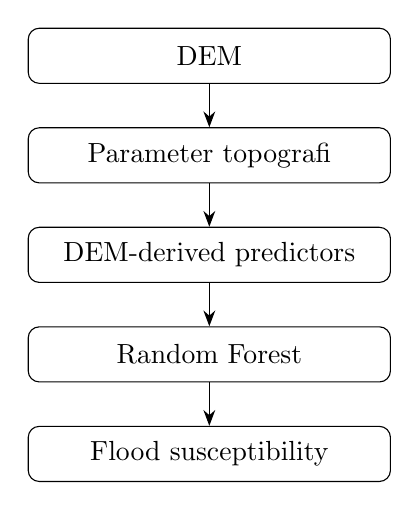
\begin{tikzpicture}[node distance=0.55cm,
  block/.style={draw, rounded corners, align=center, minimum width=4.6cm, minimum height=0.7cm}]
\node[block] (a) {DEM};
\node[block, below=of a] (b) {Parameter topografi};
\node[block, below=of b] (c) {DEM-derived predictors};
\node[block, below=of c] (d) {Random Forest};
\node[block, below=of d] (e) {Flood susceptibility};
\draw[-{Stealth[length=2mm]}] (a) -- (b);
\draw[-{Stealth[length=2mm]}] (b) -- (c);
\draw[-{Stealth[length=2mm]}] (c) -- (d);
\draw[-{Stealth[length=2mm]}] (d) -- (e);
\end{tikzpicture}
\end{center}

Karena penelitian ini bertujuan menguji sumber elevasi, setiap parameter yang
diturunkan dari DEM akan dihitung dengan prosedur yang sama untuk
masing-masing produk. Prediktor yang tidak berasal dari DEM dipertahankan
sama.

Daftar final prediktor \textbf{telah ditetapkan} dan dirinci lengkap pada
Subbab~3.6, terdiri atas 5 prediktor yang dihitung dari produk elevasi yang
diuji (elevasi, \textit{slope}, tiga representasi \textit{aspect}), 11
prediktor lingkungan non-DEM (hidrologi, hujan antecedent, indeks spektral),
serta 8 variabel \textit{dummy} tutupan lahan WorldCover (total 24
prediktor). Susunan dan fitur tersebut mengikuti praktik pada penelitian
acuan sekaligus ketersediaan data di Google Earth Engine
\cite{hakim2026}, sehingga setiap prediktor memiliki dasar rujukan.

\subsection{Random Forest untuk Flood Susceptibility}

Random Forest merupakan metode \textit{ensemble learning} yang membangun
sejumlah \textit{decision tree} dan menggabungkan hasilnya untuk memperoleh
prediksi \cite{breiman2001}. Metode ini banyak digunakan pada pemodelan
spasial karena mampu menangani hubungan nonlinier dan interaksi
antarvariabel.

Dalam penelitian sebelumnya \cite{hakim2026}, Random Forest menghasilkan
kinerja tertinggi di antara tujuh model yang dibandingkan berdasarkan
ROC-AUC (\textit{Area Under the Receiver Operating Characteristic} curve),
meskipun perbedaan dengan beberapa model teratas tidak signifikan secara
statistik.

Oleh karena itu, penelitian ini menggunakan Random Forest sebagai
\textbf{model yang dikontrol}. Tujuannya bukan menguji kembali Random Forest
melawan model lain, tetapi mempertahankan algoritma pemodelan sehingga
faktor yang diuji dapat difokuskan pada sumber elevasi.

Secara mekanistik, setiap \textit{decision tree} dibangun pada sampel
bootstrap dari data latih (bagging), dan pada setiap titik pemisahan
simpul hanya sebagian kecil variabel yang dipertimbangkan (\textit{random
subspace}) \cite{breiman2001}. Kedua sumber kerandoman itu menegaskan bahwa
pohon-pohon yang dibangun relatif tidak berkorelasi satu sama lain, sehingga
pengagregasian rata-rata antarpohon mampu menurunkan varians prediksi.
Keluaran model berupa probabilitas banjir yang dihitung dari proporsi
suara kelas antarpohon, dan probabilitas tersebut yang kemudian dipetakan
sebagai \textit{susceptibility}.

\subsection{Sensitivitas Sumber Elevasi dalam Pemodelan Banjir}

Studi Meadows dkk.\ menunjukkan bahwa produk DEM global memiliki
karakteristik galat yang berbeda dan bahwa pengaruh tersebut dapat berkaitan
dengan tutupan lahan, slope, dan kondisi medan \cite{meadows2024}. Tique
dkk.\ juga menunjukkan bahwa perubahan DEM dan metode hidrologi dapat
menghasilkan perbedaan pada \textit{flood susceptibility mapping} di Nigeria
\cite{Tique2026}. Pengaruh pilihan DEM juga dilaporkan pada pemodelan banjir
berbasis hidrolika \cite{fatdillah2022,fikri2026}.

Namun, penelitian yang sekaligus mengubah beberapa komponen dapat
menyulitkan interpretasi mengenai faktor mana yang sebenarnya menyebabkan
perubahan hasil. Oleh karena itu, penelitian ini menggunakan desain
eksperimen terkontrol:

\begin{center}
\textbf{Sumber elevasi berubah, sedangkan komponen lainnya dipertahankan.}
\end{center}

Secara sederhana, tiga eksperimen yang dibangun adalah:

\begin{center}
\begin{tabular}{ccc}
Eksperimen A: SRTM & Eksperimen B: GLO-30 & Eksperimen C: AW3D30 \\
$\downarrow$ & $\downarrow$ & $\downarrow$ \\
RF & RF & RF \\
$\downarrow$ & $\downarrow$ & $\downarrow$ \\
susceptibility & susceptibility & susceptibility \\
\end{tabular}
\end{center}

Perbedaan ketiga output kemudian digunakan untuk mengukur
\textit{DEM-source sensitivity}.

Pengukuran sensitivitas tersebut menuntut kehati-hatian evaluasi. Titik
sampel yang saling berdekatan dalam ruang geografis cenderung memiliki
nilai prediktor dan label yang serupa (autokorelasi spasial), sehingga
pemisahan latih-uji yang dilakukan secara acak pada tingkat titik
cenderung memberi estimasi performa yang terlalu optimis
\cite{roberts2017,ploton2020}. Oleh karena itu, uji ketahanan hasil pada
penelitian ini menempatkan penilaian spasial sebanding dengan penilaian
performa: metrik performa dilengkapi validasi silang spasial berbasis blok,
sedangkan selisih performa antar-DEM dievaluasi melalui resampling pada
tingkat blok dilengkapi interval kepercayaan (Subbab~3.8).

\subsection{Tutupan Lahan sebagai Stratifikasi}

Kesalahan dan karakteristik produk elevasi dapat berbeda menurut kondisi
permukaan. Meadows dkk.\ menunjukkan bahwa \textit{land cover} merupakan
faktor penting yang menjelaskan variasi galat elevasi, terutama pada area
berhutan \cite{meadows2024}.

Oleh karena itu, ESA WorldCover digunakan bukan sebagai perlakuan utama,
tetapi sebagai \textbf{variabel stratifikasi} \cite{zanaga2021}. Tujuannya
adalah menjawab pertanyaan berikut:

\begin{quote}
Apakah sensitivitas hasil \textit{susceptibility} terhadap pergantian DEM
sama pada seluruh tutupan lahan?
\end{quote}

Dengan demikian, analisis tidak berhenti pada perbandingan tiga peta secara
keseluruhan.

\subsection{Penelitian Terdahulu}

Tabel~\ref{tab:prior} merangkum penelitian yang paling relevan beserta
posisi penelitian ini terhadap masing-masing studi.

\begin{table}[ht]
\centering
\caption{Penelitian terdahulu yang relevan.}
\label{tab:prior}
\begin{adjustbox}{max width=\textwidth}
\begin{tabular}{>{\raggedright}p{2.6cm}
                >{\raggedright}p{3.6cm}
                >{\raggedright}p{3.8cm}
                >{\raggedright\arraybackslash}p{3.8cm}}
\toprule
\textbf{Penelitian} & \textbf{Fokus} & \textbf{Yang Diadopsi} & \textbf{Modifikasi pada penelitian ini} \\
\midrule
Fatdillah dkk.\ (2022) \cite{fatdillah2022} & Pengaruh DEM terhadap \textit{flood modelling} & Gagasan bahwa input elevasi dapat memengaruhi hasil banjir & Diuji dalam kerangka \textit{machine learning} terkontrol \\
Meadows dkk.\ (2024) \cite{meadows2024} & Perbandingan global produk DEM & Dasar bahwa produk elevasi mempunyai karakteristik/galat berbeda & Dampak DEM ditelusuri sampai output \textit{susceptibility} \\
Yuwono dkk.\ (2024) \cite{yuwono2024} & Perbandingan DEM pada pemodelan hidrolika banjir Semarang & Konteks perbandingan DEM di wilayah studi & Diuji pada kerangka \textit{machine learning} \\
Verdyansyah dkk.\ (2025) \cite{verdyansyah2025} & \textit{Machine learning} + banjir di Kabupaten Demak & Konteks pemodelan banjir berbasis \textit{machine learning} lokal & Sumber elevasi divariasikan secara sistematis \\
Hakim dkk.\ (SMDS) \cite{hakim2026} & Sentinel-1 + tujuh model untuk \textit{flood susceptibility} Semarang--Demak & \textit{Flood inventory} Sentinel-1 dan baseline Random Forest & RF dipertahankan dan DEM dijadikan faktor eksperimen \\
Fikri dkk.\ (2026) \cite{fikri2026} & Pengaruh karakteristik/resolusi DEM terhadap \textit{flood modelling} & Sensitivitas output terhadap data elevasi & Fokus pada \textit{source sensitivity} dan \textit{spatial susceptibility} \\
Studi Tique dkk.\ (2026) \cite{Tique2026} & Multi-DEM + ML \textit{flood susceptibility} & Bukti empiris bahwa pilihan DEM berpengaruh & Variabel lain dikontrol sehingga fokus pada sumber DEM \\
\bottomrule
\end{tabular}
\end{adjustbox}
\end{table}

Studi Tique dkk.\ merupakan rujukan terbaru yang paling relevan karena
secara eksplisit membandingkan empat DEM, beberapa metode hidrologi, dan tiga
model \textit{machine learning}. Penelitian tersebut menunjukkan bahwa
kombinasi Copernicus DEM dengan metode hidrologi tertentu menghasilkan
performa tertinggi, sekaligus menunjukkan bahwa variasi pilihan DEM
dapat memengaruhi hasil \textit{susceptibility} \cite{Tique2026}.

Namun, perbedaan pada gilirannya memperlihatkan posisi penelitian ini dengan
lebih jelas: penelitian
Tique dkk.\ mengubah \textbf{DEM + metode hidrologi + model ML}, sedangkan
penelitian ini mempertahankan model dan komponen lain secara tetap agar
perubahan output lebih langsung dikaitkan dengan \textbf{sumber elevasi}.
Perbedaan tersebut menjadi dasar kebaruan penelitian ini.

\subsection{Kerangka Teori}

Kerangka teori penelitian dapat dirumuskan sebagai rangkaian sebab-akibat
berikut:

\begin{figure}[ht]
\centering
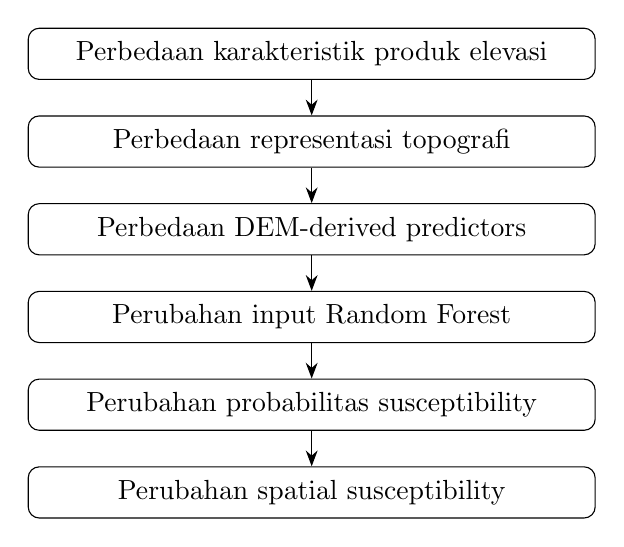
\begin{tikzpicture}[node distance=0.45cm,
  block/.style={draw, rounded corners, align=center, minimum width=7.2cm, minimum height=0.65cm}]
\node[block] (a) {Perbedaan karakteristik produk elevasi};
\node[block, below=of a] (b) {Perbedaan representasi topografi};
\node[block, below=of b] (c) {Perbedaan DEM-derived predictors};
\node[block, below=of c] (d) {Perubahan input Random Forest};
\node[block, below=of d] (e) {Perubahan probabilitas susceptibility};
\node[block, below=of e] (f) {Perubahan spatial susceptibility};
\draw[-{Stealth[length=2mm]}] (a) -- (b);
\draw[-{Stealth[length=2mm]}] (b) -- (c);
\draw[-{Stealth[length=2mm]}] (c) -- (d);
\draw[-{Stealth[length=2mm]}] (d) -- (e);
\draw[-{Stealth[length=2mm]}] (e) -- (f);
\end{tikzpicture}
\caption{Kerangka teori rangkaian sebab-akibat dari sumber produk elevasi
sampai keluaran \textit{flood susceptibility}.}
\label{fig:kerangka-teori}
\end{figure}

Kerangka pada Gambar~\ref{fig:kerangka-teori} menjelaskan bahwa sumber
produk elevasi menjadi simpul paling awal rantai sebab-akibat. Selanjutnya,
kondisi permukaan digunakan untuk menjelaskan variasinya: perbedaan
spasial \textit{susceptibility} dipetakan terhadap kelas tutupan lahan ESA
WorldCover, sehingga sensitivitas sumber elevasi dapat dibandingkan antar
tutupan lahan.

\subsection{Kerangka Berpikir}

\begin{figure}[ht]
\centering
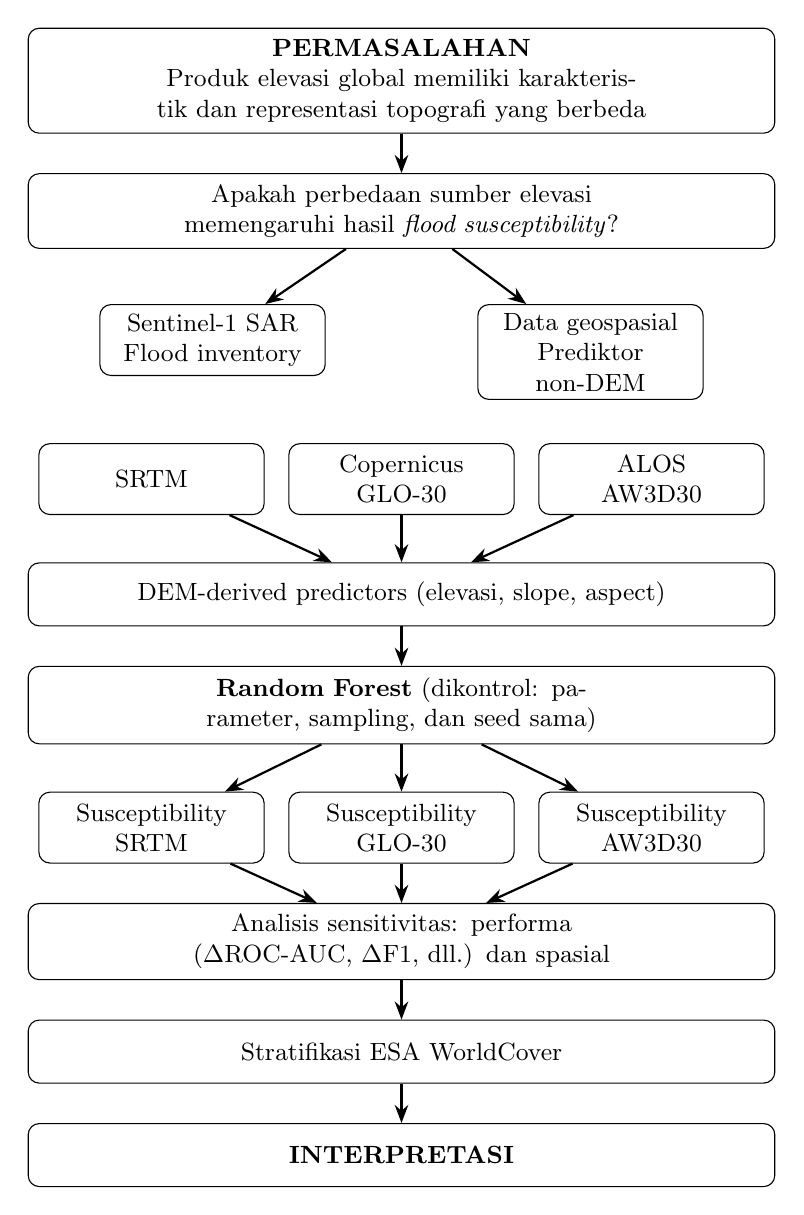
\begin{tikzpicture}[
  font=\small,
  block/.style={draw, rounded corners, align=center, text width=9.2cm,
                minimum height=0.8cm, inner sep=4pt},
  small/.style={draw, rounded corners, align=center, text width=2.65cm,
                minimum height=0.9cm, inner sep=3pt},
  arrow/.style={-{Stealth[length=2.3mm]}, thick},
]
\node[block] (prob) {\textbf{PERMASALAHAN}\\
  Produk elevasi global memiliki karakteristik dan representasi topografi yang berbeda};
\node[block, below=5mm of prob] (q)
  {Apakah perbedaan sumber elevasi memengaruhi hasil \textit{flood susceptibility}?};

\node[small, below=7mm of q, xshift=-2.4cm] (s1)
  {Sentinel-1 SAR\\Flood inventory};
\node[small, below=7mm of q, xshift=2.4cm] (geo)
  {Data geospasial\\Prediktor non-DEM};

\coordinate (inputbottom) at ($(s1.south)!0.5!(geo.south)$);
\node[small, below=7mm of inputbottom] (d2) {Copernicus\\GLO-30};
\node[small, left=3mm of d2] (d1) {SRTM};
\node[small, right=3mm of d2] (d3) {ALOS\\AW3D30};

\node[block, below=6mm of d2] (dempred)
  {DEM-derived predictors (elevasi, slope, aspect)};
\node[block, below=5mm of dempred] (rf)
  {\textbf{Random Forest} (dikontrol: parameter, sampling, dan seed sama)};

\node[small, below=6mm of rf] (m2) {Susceptibility\\GLO-30};
\node[small, left=3mm of m2] (m1) {Susceptibility\\SRTM};
\node[small, right=3mm of m2] (m3) {Susceptibility\\AW3D30};

\node[block, below=5mm of m2] (sens)
  {Analisis sensitivitas: performa ($\Delta$ROC-AUC, $\Delta$F1, dll.) dan spasial};
\node[block, below=5mm of sens] (wc) {Stratifikasi ESA WorldCover};
\node[block, below=5mm of wc] (int) {\textbf{INTERPRETASI}};
% Panah
\draw[arrow] (prob) -- (q);
\draw[arrow] (q) -- (s1);
\draw[arrow] (q) -- (geo);
\draw[arrow] (d1) -- (dempred);
\draw[arrow] (d2) -- (dempred);
\draw[arrow] (d3) -- (dempred);
\draw[arrow] (dempred) -- (rf);
\draw[arrow] (rf) -- (m1);
\draw[arrow] (rf) -- (m2);
\draw[arrow] (rf) -- (m3);
\draw[arrow] (m1) -- (sens);
\draw[arrow] (m2) -- (sens);
\draw[arrow] (m3) -- (sens);
\draw[arrow] (sens) -- (wc);
\draw[arrow] (wc) -- (int);
\end{tikzpicture}
\caption{Kerangka berpikir penelitian.}
\label{fig:kerangka}
\end{figure}

Alur penelitian pada Gambar~\ref{fig:kerangka} menunjukkan bahwa
\textit{flood inventory} Sentinel-1 dan prediktor non-DEM berada di luar
perlakuan, sehingga satu-satunya komponen yang bervariasi adalah sumber
produk elevasi. Ketiga peta \textit{susceptibility} yang dihasilkan kemudian
dibandingkan pada tingkat performa dan spasial, sebelum dianalisis lebih
lanjut menurut kelas tutupan lahan.

%==================================================================
% BAB III
%==================================================================

\clearpage
\section{Metode Penelitian}

\subsection{Pendekatan dan Desain Penelitian}

Penelitian ini menggunakan pendekatan kuantitatif dengan desain
\textbf{eksperimen terkontrol}. Eksperimen dilakukan untuk menguji
sensitivitas hasil \textit{flood susceptibility mapping} terhadap pemilihan
produk elevasi.

Faktor perlakuan dalam penelitian adalah \textbf{sumber produk elevasi},
dengan tiga level perlakuan:

\begin{enumerate}
\item SRTM;
\item Copernicus DEM GLO-30;
\item ALOS AW3D30.
\end{enumerate}

Random Forest digunakan sebagai model yang sama pada ketiga eksperimen.
\textit{Flood inventory}, wilayah penelitian, prediktor non-elevasi, prosedur
preprocessing, prosedur sampling, dan prosedur evaluasi dipertahankan sama.
Dengan demikian, perbedaan hasil antarperlakuan terutama ditujukan untuk
merepresentasikan pengaruh perubahan sumber elevasi. Ringkasan desain
eksperimen disajikan pada Tabel~\ref{tab:desain}.

\begin{table}[ht]
\centering
\caption{Desain eksperimen penelitian.}
\label{tab:desain}
\begin{tabular}{ll}
\toprule
\textbf{Komponen} & \textbf{Kondisi} \\
\midrule
Faktor perlakuan & Produk elevasi \\
Level 1 & SRTM \\
Level 2 & Copernicus DEM GLO-30 \\
Level 3 & ALOS AW3D30 \\
Model ML & Random Forest \\
Flood inventory & Sama \\
Wilayah & Sama \\
Prediktor non-DEM & Sama \\
Prosedur preprocessing & Sama \\
Prosedur sampling & Sama \\
Prosedur evaluasi & Sama \\
Analisis tambahan & Stratifikasi WorldCover \\
\bottomrule
\end{tabular}
\end{table}

\subsection{Wilayah Penelitian}

Wilayah penelitian berada pada kawasan pesisir Semarang--Demak, Jawa Tengah,
Indonesia. Wilayah tersebut dipilih karena memiliki karakteristik dataran
rendah, kawasan pesisir, kawasan pertanian dan terbangun, serta riwayat
kejadian banjir yang membuat sensitivitas representasi topografi menjadi
relevan untuk dikaji \cite{marfai2008,Husnayaen2018,Sakina2025}.

Batas wilayah penelitian mengikuti area pesisir Kota Semarang dan Kabupaten
Demak (administrasi provinsi Jawa Tengah tingkat 2, FAO GAUL) yang sama
dengan yang digunakan pada penelitian SMDS sebelumnya agar konteks
wilayah dan sumber data dapat dibandingkan secara konsisten
\cite{hakim2026}.

\subsection{Data dan Sumber Data}

\begin{table}[ht]
\centering
\caption{Matriks data penelitian: sifat sumber, bentuk keluaran, unit
pengukuran, produsen, katalog Google Earth Engine, dan fungsi dalam
penelitian.}
\label{tab:data}
\small
\begin{adjustbox}{max width=\textwidth}
\begin{tabular}{>{\raggedright}p{2.5cm}>{\raggedright}p{2.5cm}>{\raggedright}p{1.55cm}>{\raggedright}p{1.4cm}>{\raggedright}p{3.55cm}>{\raggedright\arraybackslash}p{2.2cm}}
\toprule
\textbf{Data} & \textbf{Jenis/sifat} & \textbf{Bentuk \& resolusi} & \textbf{Unit} & \textbf{Produsen; ID katalog GEE} & \textbf{Fungsi (RM)} \\
\midrule
Sentinel-1 GRD (\textit{Ground Range Detected}) & Radar SAR pita-C; pra \& pasca kejadian & Citra GRD/IW 10 m & dB & ESA Copernicus; \texttt{COPERNICUS/\allowbreak S1\_GRD} & Pembentukan \textit{flood inventory} (RM 2, RM 4) \\
SRTM & Radar C-band interferometri; DSM & Grid 30 m & m & NASA/USGS; \texttt{USGS/\allowbreak SRTMGL1\_003} & Perlakuan elevasi 1 (RM 1, RM 2) \\
Copernicus DEM GLO-30 & Radar bistatik pita-X TanDEM-X; DSM & Grid 30 m & m & ESA Copernicus (GMES); \texttt{COPERNICUS/\allowbreak DEM/\allowbreak GLO30} & Perlakuan elevasi 2 (RM 1, RM 2) \\
ALOS AW3D30 (V4.1) & Stereo fotogrametri optik PRISM; DSM & Grid 30 m & m & JAXA; \texttt{JAXA/\allowbreak ALOS/\allowbreak AW3D30/\allowbreak V4\_1} & Perlakuan elevasi 3 (RM 1, RM 2) \\
MERIT Hydro & Turunan DEM aplikasi hidrologi & Grid 90 m & m / log & Univ. Tokyo (Yamazaki dkk.); \texttt{MERIT/\allowbreak Hydro/\allowbreak v1\_0\_1} & HAND, aliran hulu, lebar \& jarak sungai (RM 2) \\
JRC Global Surface Water & Rekap air permukaan 1984--2021 & Citra raster; pita \textit{occ} & \% & Komisi Eropa (JRC); \texttt{JRC/\allowbreak GSW1\_4/\allowbreak GlobalSurfaceWater} & Masking air permanen; jarak air (RM 2, RM 4) \\
CHIRPS harian & Klimatologi hujan IR + stasiun & Grid $0{,}05^{\circ}$ (5,5 km) & mm/hari & UCSB CHG; \texttt{UCSB-CHG/\allowbreak CHIRPS/\allowbreak DAILY} & Hujan antecedent 7 \& 30 hari (RM 2) \\
Sentinel-2 SR (L2A) & Citra permukaan optik multispektral & Citra 10--60 m & refl.\ (SR) & ESA Copernicus; \texttt{COPERNICUS/\allowbreak S2\_SR\_HARMONIZED} & NDVI, NDWI, MNDWI, NDBI (RM 2) \\
ESA WorldCover (v200) & Klasifikasi tutupan lahan 11 kelas & Citra 10 m & kode kelas & ESA; \texttt{ESA/\allowbreak WorldCover/\allowbreak v200} & Variabel \textit{dummy} + stratifikasi (RM 2, RM 3, RM 4) \\
\bottomrule
\end{tabular}
\end{adjustbox}
\end{table}

\subsection{Perangkat Penelitian}

Penelitian utama dilakukan menggunakan Google Earth Engine untuk akuisisi
dan preprocessing data spasial \cite{gorelick2017}. Pengolahan data dan
pemodelan Random Forest dapat dilakukan menggunakan lingkungan
Python/Google Colab apabila diperlukan.

Penggunaan Google Earth Engine dipilih karena menyediakan akses terhadap
berbagai dataset penginderaan jauh dan geospasial pada lingkungan komputasi
yang sama, sehingga ketiga produk elevasi dapat diolah dengan prosedur yang
konsisten.

\subsection{Pembentukan Flood Inventory}

Flood inventory dibentuk menggunakan citra Sentinel-1 SAR. Tahapan utamanya:

\begin{enumerate}
\item penyusunan komposit Sentinel-1 pra-kejadian dan pasca-kejadian;
\item preprocessing citra SAR;
\item perhitungan perubahan \textit{backscatter} antarperiode;
\item identifikasi area yang mengalami perubahan konsisten dengan genangan;
\item masking perairan permanen menggunakan JRC Global Surface Water
\cite{pekel2016};
\item pembentukan label \textit{flood}/\textit{non-flood}.
\end{enumerate}

Pendekatan ini mengikuti prinsip pembentukan label banjir berbasis perubahan
Sentinel-1 yang digunakan dalam penelitian SMDS sebelumnya \cite{hakim2026}
serta praktik \textit{change detection} yang terdokumentasi
\cite{islammeng2022,unspider2024}. Parameter threshold dan kejadian yang
digunakan telah ditetapkan secara final dan diterapkan identik pada ketiga
eksperimen:

\begin{itemize}
\item komposit median polarisasi VH untuk periode pra-kejadian
(25 Februari--12 Maret 2024) dan pasca-kejadian (15--31 Maret 2024);
\item kriteria piksel banjir: rasio daya \textit{backscatter} pra-kejadian
terhadap pasca-kejadian $>1{,}25$ dan daya VH pasca-kejadian $<-18$~dB;
\item piksel berada di luar perairan permanen JRC Global Surface Water
(\textit{occurrence} $\geq 80\%$);
\item kemiringan lereng SRTM $<5^{\circ}$ untuk menyaring artefak geometrik
radar \cite{hakim2026};
\item penyaringan konektivitas spasial minimum 8 piksel.
\end{itemize}

Penetapan nilai threshold mengikuti konfigurasi penelitian acuan
\cite{hakim2026} supaya hasil dapat dibandingkan secara langsung, bukan
ditetapkan secara arbitrer. Karena label dibentuk satu kali dan dipakai
sama pada ketiga eksperimen, label tidak menjadi sumber variasi
antarperlakuan.

Kriteria kemiringan lereng di bawah $5^{\circ}$ bertujuan menyingkirkan
artefak geometris radar pita-C pada area berlereng curam, seperti
\textit{layover} dan \textit{foreshortening}, bukan membatasi domain pesisir.
Karena acuan lereng berasal dari SRTM, pengaruh pilihan ini terhadap
komposisi label diperiksa pada Subbab~4.2.

\subsection{Pembentukan Prediktor}

Prediktor penelitian dibagi menjadi dua kelompok.

\subsubsection{DEM-derived predictors}

Prediktor yang diperoleh dari setiap produk elevasi terdiri atas lima fitur
dengan prosedur ekstraksi yang identik dihitung menggunakan modul terain
Google Earth Engine (\texttt{ee.Terrain}):

\begin{itemize}
\item \textit{elevation} (elevasi permukaan, meter);
\item \textit{slope} (kemiringan lereng, derajat);
\item \textit{aspect}\textsubscript{sin} (komponen sinus arah lereng);
\item \textit{aspect}\textsubscript{cos} (komponen kosinus arah lereng);
\item \textit{aspect}\textsubscript{valid} (indikator validitas arah lereng).
\end{itemize}

Arah lereng (\textit{aspect}) pada dasarnya dinyatakan dalam sudut $0^{\circ}$
sampai $360^{\circ}$ sehingga mengandung diskontinuitas melingkar pada batas
$0^{\circ}$/$360^{\circ}$. Untuk menghindari kesalahan interprestasi nilai
sudut oleh model, \textit{aspect} direpresentasikan melalui dekomposisi
sinus dan kosinusnya, serta satu indikator biner yang menandai piksel dengan
arah lereng terdefinisi; pada daerah datar, arah lereng tidak terdefinisi
sehingga kasus tersebut dipisahkan secara eksplisit oleh indikator. Kelima fitur tersebut
diulang identik untuk masing-masing produk elevasi yang diuji, sehingga jumlah
prediktor yang diturunkan dari DEM sama pada ketiga konfigurasi.

Ketiga produk DEM diproses menggunakan prosedur yang sama, termasuk
penyelarasan grid, clipping wilayah penelitian, serta dokumentasi perbedaan
acuan vertikal (EGM96 pada SRTM versus EGM2008 pada Copernicus dan ALOS;
keduanya merupakan \textit{Earth Gravitational Model})
yang kritis pada dataran pesisir rendah.

\subsubsection{Prediktor non-DEM dan dummy tutupan lahan}

Prediktor yang tidak bergantung pada sumber DEM dipertahankan sama pada
ketiga eksperimen dan mengikuti set pada penelitian acuan \cite{hakim2026}.
Sebelas prediktor non-DEM terdiri atas:

\begin{itemize}
\item variabel hidrologi dari MERIT Hydro \cite{yamazaki2019}: HEIGHT
Above Nearest Drainage (HAND), logaritma luas aliran hulu
(\textit{upstream drainage area}), lebar sungai (\textit{river width}), dan
jarak ke sungai terdekat;
\item jarak ke badan air permanen JRC Global Surface Water
\cite{pekel2016};
\item curah hujan antecedent CHIRPS \cite{funk2015} berupa akumulasi 7 hari
dan 30 hari sebelum kejadian;
\item indeks spektral Sentinel-2 \cite{saha2021}: NDVI
(\textit{Normalized Difference Vegetation Index}), NDWI
(\textit{Normalized Difference Water Index}), MNDWI (\textit{Modified
Normalized Difference Water Index}), dan NDBI (\textit{Normalized
Difference Built-up Index}).
\end{itemize}

Delapan variabel \textit{dummy} tutupan lahan dihasilkan dari
kategorisasi kelas ESA WorldCover \cite{zanaga2021} (kode 10 tutupan pohon,
30 padang rumput, 40 lahan pertanian, 50 kawasan terbangun, 60 lahan tanpa
vegetasi, 80 badan air, 90 lahan basah herba, dan 95 mangrove), dengan kelas
tutupan semak belukar (kode 20) sebagai kategori acuan yang tidak
dimodelkan. Dengan demikian, jumlah total fitur tertutup menjadi
$5+11+8=24$ variabel prediktor.

\subsection{Eksperimen Random Forest Terkontrol}

Eksperimen dilakukan sebanyak tiga perlakuan:

\begin{description}
\item[Eksperimen 1] SRTM $\rightarrow$ DEM-derived predictors $\rightarrow$
prediktor non-DEM yang sama $\rightarrow$ Random Forest $\rightarrow$
\textit{Susceptibility Map} SRTM.
\item[Eksperimen 2] Copernicus GLO-30 $\rightarrow$ DEM-derived predictors
$\rightarrow$ prediktor non-DEM yang sama $\rightarrow$ Random Forest
$\rightarrow$ \textit{Susceptibility Map} GLO-30.
\item[Eksperimen 3] ALOS AW3D30 $\rightarrow$ DEM-derived predictors
$\rightarrow$ prediktor non-DEM yang sama $\rightarrow$ Random Forest
$\rightarrow$ \textit{Susceptibility Map} AW3D30.
\end{description}

Ketiga eksperimen menggunakan \textit{flood inventory} yang sama sehingga
label tidak menjadi sumber variasi antarperlakuan. Demikian pula \textit{seed}
sampling, pembagian data latih-uji, dan parameter Random Forest dipertahankan
identik antarperlakuan.

Konfigurasi Random Forest yang digunakan adalah sebagai berikut. Peta
probabilitas spasial dibangun di Google Earth Engine menggunakan
\texttt{ee.Classifier.smileRandomForest} dengan 300 pohon, sedangkan
evaluasi metrik dilakukan pada implementasi Random Forest scikit-learn
dengan 400 pohon, tebal minimum daun (\textit{minimum samples leaf}) 2,
pemberatan kelas \textit{balanced} (\texttt{class\_weight}), dan
\textit{random state} yang disamakan antarperlakuan. Pengambilan sampel
dilakukan terstratifikasi sebanyak 2.978 titik per kelas
(\textit{seed}~42) mengikuti jumlah populasi berlabel pada kedua kelas,
kemudian data dibagi 75\% latih dan 25\% uji dan diperlakukan identik pada
ketiga perlakuan. Estimasi ketahanan hasil terhadap efek autokorelasi
spasial dan pilihan \textit{seed} dilaporkan melalui pengecekan dengan
validasi silang spasial dan bootstrap blok pada Subbab~3.8.

\subsection{Evaluasi Model}

Evaluasi dilakukan terhadap kemampuan model membedakan lokasi berlabel
banjir dan non-banjir menggunakan data pengujian yang sama secara
metodologis.

Metrik yang digunakan meliputi:

\begin{itemize}
\item ROC-AUC;
\item accuracy;
\item precision;
\item recall;
\item F1-score.
\end{itemize}

Pemilihan metrik tersebut mengikuti karakteristik masalah sebagai
klasifikasi biner dan praktik evaluasi pada penelitian \textit{flood
susceptibility} berbasis \textit{machine learning}. Penelitian sebelumnya
juga menggunakan metrik-metrik tersebut untuk mengevaluasi model
\cite{hakim2026}. Ambang klasifikasi ditentukan menggunakan indeks Youden
dihitung pada kurva ROC (\textit{Receiver Operating Characteristic})
\cite{youden1950}.

Namun evaluasi tidak berhenti pada pertanyaan ``model mana yang memiliki
accuracy paling tinggi?'', karena ketiga model dibangun dengan konfigurasi
identik. Pertanyaan
utamanya adalah: \textbf{seberapa besar output model berubah ketika sumber
DEM diganti?}

Karena titik sampel yang berdekatan cenderung mengandung autokorelasi
spasial, evaluasi performa diperkuat tiga skema pengecekan yang identik pada ketiga
perlakuan \cite{roberts2017,ploton2020}:

\begin{itemize}
\item \textbf{validasi silang spasial 4-\textit{fold}}: ruang geografis
dibagi menjadi 16 blok berdasarkan kuantil lintang dan bujur, empat blok
diambil bergiliran sebagai blok uji, dan metrik dihitung dari probabilitas
piksel uji;
\item \textbf{bootstrap blok}: selisih ROC-AUC antarproduk diresample
1.000 kali dengan pengembalian pada tingkat 16 blok yang sama, dan
interval kepercayaan 95\% disajikan; skema ini menguji apakah selisih
performa antarproduk berbeda dari nol;
\item \textbf{pengujian multi-\textit{seed}}: lima nilai \textit{seed}
(42, 100, 2024, 7, dan 99) diulang dari nol, termasuk sampling, ekstraksi
fitur, dan pembagian data, untuk memeriksa konsistensi arah peringkat
antarproduk.
\end{itemize}

\subsection{Analisis Sensitivitas}

Analisis sensitivitas dilakukan dengan membandingkan output tiga eksperimen.
Perbandingan dilakukan pada dua tingkat.

\subsubsection{Sensitivitas performa}

Membandingkan perubahan metrik antarperlakuan:

\begin{quote}
$\Delta$ROC-AUC, $\Delta$F1, $\Delta$precision, dan $\Delta$recall.
\end{quote}

\subsubsection{Sensitivitas spasial}

Membandingkan:

\begin{itemize}
\item probabilitas \textit{susceptibility};
\item kelas \textit{susceptibility};
\item luas area setiap kelas;
\item kesesuaian spasial antarhasil (\textit{spatial agreement}).
\end{itemize}

Dengan demikian, penelitian tidak hanya dapat mengatakan bahwa suatu produk
lebih akurat daripada yang lain, tetapi juga dapat menjawab pertanyaan
\textbf{di mana} hasil \textit{susceptibility} berubah ketika DEM diganti.

\subsection{Stratifikasi Berdasarkan Tutupan Lahan}

ESA WorldCover digunakan untuk membagi wilayah penelitian berdasarkan kelas
tutupan lahan \cite{zanaga2021}. Kemudian perubahan \textit{susceptibility}
akibat pergantian DEM dihitung pada masing-masing kelompok, misalnya
kawasan terbangun, pertanian, dan vegetasi.

Analisis ini dilakukan untuk mengetahui apakah sensitivitas sumber elevasi
menunjukkan pola yang berbeda pada jenis permukaan tertentu. Dasarnya adalah
temuan Meadows dkk.\ bahwa \textit{land cover} merupakan salah satu faktor
utama yang berkaitan dengan variasi galat pada produk DEM global
\cite{meadows2024}.

\subsection{Tahapan Penelitian}

\begin{table}[ht]
\centering
\caption{Tahapan penelitian.}
\label{tab:tahapan}
\begin{adjustbox}{max width=\textwidth}
\begin{tabular}{clp{5.4cm}p{4.6cm}}
\toprule
\textbf{Tahap} & \textbf{Kegiatan} & \textbf{Output} & \textbf{Orientasi RM} \\
\midrule
1 & Studi literatur & Dasar teori dan metode & Seluruh RM \\
2 & Penentuan AOI (\textit{area of interest}) & Wilayah penelitian & RM 1, RM 3, RM 4 \\
3 & Akuisisi Sentinel-1 & Data SAR & RM 2, RM 4 \\
4 & Pembentukan \textit{flood inventory} & Label \textit{flood/non-flood} & RM 2, RM 3, RM 4 \\
5 & Akuisisi tiga DEM & SRTM, GLO-30, AW3D30 & RM 1 \\
6 & Prapemrosesan DEM & DEM siap digunakan & RM 1 \\
7 & Ekstraksi prediktor turunan DEM & Prediktor topografi & RM 1 \\
8 & Penyusunan prediktor & Dataset pemodelan & RM 1, RM 2 \\
9 & Eksperimen Random Forest SRTM & Peta \textit{flood susceptibility} SRTM & RM 2 \\
10 & Eksperimen Random Forest GLO-30 & Peta \textit{flood susceptibility} GLO-30 & RM 2 \\
11 & Eksperimen Random Forest AW3D30 & Peta \textit{flood susceptibility} AW3D30 & RM 2 \\
12 & Evaluasi model & Metrik performa & RM 2, RM 3 \\
13 & Analisis sensitivitas spasial & Perubahan spasial peta & RM 3, RM 4 \\
14 & Stratifikasi WorldCover & Sensitivitas menurut tutupan lahan & RM 3, RM 4 \\
15 & Interpretasi & Kesimpulan sensitivitas DEM & Seluruh RM \\
\bottomrule
\end{tabular}
\end{adjustbox}
\end{table}

%==================================================================
% BAB IV
%==================================================================

\clearpage
\section{Hasil dan Pembahasan}

Bab ini menyajikan hasil eksperimen terkontrol untuk satu kejadian banjir pada
satu wilayah kajian (\textit{Area of Interest}), dengan satu sampel induk
(\textit{master sample}) acak yang terdiri atas 2.978 titik banjir dan 2.978
titik non-banjir ($n=5.956$). Sampel induk dipertahankan identik pada ketiga
konfigurasi produk elevasi. Setiap model Random Forest \cite{breiman2001}
menggunakan 24 prediktor, yaitu 11 prediktor non-DEM, 8 variabel
\textit{dummy} tutupan lahan, dan 5 prediktor topografi yang diturunkan dari
masing-masing produk DEM yang diuji. Pengolahan dilakukan menggunakan Google
Earth Engine dan lingkungan komputasi Kaggle (GPU T4). Statistik spasial pada
Subbab~4.5 dan~4.6 diturunkan dari eksperimen utama, dan ketahanan hasil
terhadap pembangkit acak diperiksa dengan lima nilai \textit{seed} yang
berbeda (Subbab~4.4).

Satu temuan metodologis perlu dicatat sejak awal. Pada uji awal, titik
non-banjir hanya terambil dari zona di sekitar perairan permanen JRC karena
pita \textit{occurrence} bersifat jarang (\textit{sparse}), sehingga piksel
daratan tanpa rekaman air ikut tersingkir saat \textit{masking}. Rata-rata
elevasi sampel non-banjir pada uji tersebut hanya $4{,}15$~m, jauh di bawah
rata-rata elevasi wilayah kajian sebesar $42{,}7$~m. Setelah \textit{masking}
diperbaiki dengan fungsi \texttt{unmask(0)}, populasi kandidat non-banjir
mencakup sekitar 97,9\% wilayah kajian. ROC-AUC validasi silang spasial pada
domain sempit di sekitar perairan hanya sekitar $0{,}70$, sedangkan pada
seluruh wilayah kajian mencapai $0{,}870$ hingga $0{,}890$. Selisih sekitar
$0{,}17$ ini jauh melampaui selisih antarproduk elevasi dan menunjukkan bahwa
estimasi performa sangat dipengaruhi desain sampel kelas non-banjir. Seluruh
hasil berikutnya berasal dari desain yang telah diperbaiki.

\subsection{Hasil Karakteristik Produk Elevasi}

Analisis statistik deskriptif pada grid resolusi 30~meter menunjukkan bahwa
ketiga produk elevasi global merepresentasikan karakteristik bentang lahan
yang sejalan, yaitu kombinasi dataran rendah pesisir di bagian utara dan
perbukitan di bagian selatan, dengan selisih vertikal yang relatif kecil.
Rata-rata elevasi pada wilayah penelitian tercatat sebesar $40{,}62$~m untuk
SRTM, $39{,}06$~m untuk Copernicus DEM GLO-30, dan $41{,}36$~m untuk ALOS
AW3D30, dengan nilai median masing-masing sebesar $8{,}50$~m, $4{,}94$~m, dan
$8{,}53$~m. Selisih (\textit{offset}) vertikal rata-rata terhadap SRTM adalah
$-1{,}56$~m pada Copernicus DEM GLO-30 dan $+0{,}39$~m pada ALOS AW3D30. Nilai
tersebut dilaporkan tanpa transformasi koreksi vertikal untuk
mendokumentasikan perbedaan datum geoid bawaan antara EGM96 pada SRTM dan
EGM2008 pada Copernicus DEM GLO-30 serta ALOS AW3D30. Sementara itu, rata-rata
kemiringan lereng (\textit{slope}) yang dihasilkan oleh masing-masing produk
adalah $3{,}03^{\circ}$ pada SRTM, $2{,}46^{\circ}$ pada Copernicus DEM GLO-30,
dan $3{,}13^{\circ}$ pada ALOS AW3D30.

\subsection{Hasil Flood Inventory}

Pembentukan \textit{flood inventory} diturunkan dari citra Sentinel-1 GRD
polarisasi VH (\textit{vertical transmit, horizontal receive}) menggunakan komposit median periode pra-kejadian
(25~Februari--12~Maret 2024) dan pasca-kejadian (15--31~Maret 2024).
Identifikasi genangan dilakukan menggunakan kriteria rasio daya
\textit{backscatter} sebelum terhadap sesudah kejadian sebesar lebih dari
$1{,}25$, nilai \textit{backscatter} pasca-kejadian kurang dari $-18$~dB,
berada di luar badan air permanen berdasarkan JRC Global Surface Water
(\textit{occurrence} $\geq 80\%$), memiliki kemiringan lereng kurang dari
$5^{\circ}$, serta memenuhi penyaringan konektivitas spasial minimum 8~piksel.
Prosedur dan parameter ini mengikuti rancangan pada penelitian acuan
\cite{hakim2026}, yang menghasilkan populasi piksel valid sebanyak 1.410.981
piksel non-banjir dan 58.573 piksel banjir. Label hasil ekstraksi ulang memiliki kecocokan 70\% terhadap 1.870 titik
sampel penelitian acuan \cite{hakim2026}. Selisih ini kemungkinan berkaitan
dengan pemrosesan ulang (\textit{reprocessing}) arsip Sentinel-1 di Google
Earth Engine. Kesetaraan dengan penelitian acuan karena itu terbatas pada
algoritma dan parameter, sedangkan perbandingan antarproduk pada
Subbab~4.4 tetap memakai himpunan label yang sama.

Evaluasi lebih lanjut terhadap karakteristik topografi pada 2.978 titik sampel
banjir menunjukkan bahwa lokasi genangan terkonsentrasi di kawasan dataran
rendah pesisir. Pada produk SRTM, median kemiringan lereng titik banjir
tercatat sebesar $1{,}35^{\circ}$ (persentil ke-99 sebesar $4{,}92^{\circ}$
dan maksimum $11{,}48^{\circ}$), sedangkan pada Copernicus DEM GLO-30 tercatat
sebesar $0{,}28^{\circ}$ (dengan 99,97\% titik berada di bawah $5^{\circ}$)
dan pada ALOS AW3D30 sebesar $0{,}96^{\circ}$ (dengan 98,76\% titik berada di
bawah $5^{\circ}$). Median elevasi pada titik-titik banjir tersebut
masing-masing adalah $3{,}0$~m untuk SRTM, $1{,}4$~m untuk Copernicus DEM
GLO-30, dan $4{,}0$~m untuk ALOS AW3D30. Mengingat selisih kemiringan lereng
antarproduk elevasi pada titik banjir tergolong kecil (median
$|\Delta\text{slope}|$ berkisar antara $0{,}85^{\circ}$ hingga $1{,}24^{\circ}$
dengan korelasi antarproduk yang rendah), kriteria penyaringan lereng di bawah
$5^{\circ}$ efektif berfungsi untuk menyingkirkan artefak geometris radar
pita-C (\textit{layover} dan \textit{foreshortening}) pada perbukitan di
bagian selatan wilayah kajian, bukan memangkas domain genangan di kawasan
pesisir. Dengan demikian, penggunaan SRTM sebagai acuan penyaringan lereng
tidak menggeser populasi label banjir secara substansial.

\subsection{Hasil Pemodelan Random Forest}

Pemodelan spasial untuk menghasilkan tiga peta probabilitas \textit{flood
susceptibility} dilakukan menggunakan algoritma \texttt{smileRandomForest}
pada Google Earth Engine dengan konfigurasi 300 pohon keputusan
(\textit{trees}) yang dilatih pada sampel induk yang sama. Probabilitas
prediksi yang dihasilkan selanjutnya dikelompokkan ke dalam lima kelas
kerawanan banjir (sangat rendah, rendah, sedang, tinggi, dan sangat tinggi)
menggunakan batas interval seragam sebesar $0{,}2$; $0{,}4$; $0{,}6$; dan
$0{,}8$ pada ketiga peta. Sementara itu, evaluasi kinerja prediktif pada skema
\textit{holdout} dilakukan menggunakan implementasi Random Forest pada pustaka
\textit{scikit-learn} (400~\textit{trees}) dengan pembagian data latih dan
data uji secara acak terstratifikasi sebesar 75:25 ($n_{\text{uji}}=1.489$).
Penentuan ambang klasifikasi optimal menggunakan indeks Youden
\cite{youden1950} yang dihitung pada data uji hanya disajikan sebagai
informasi pelaporan tambahan karena sifatnya yang cenderung optimistis,
sedangkan metrik klasifikasi utama pada Tabel~\ref{tab:metrik-holdout}
dievaluasi pada ambang baku $0{,}5$. Seluruh statistik spasial peta, yang
meliputi distribusi luas kelas, matriks transisi antarkelas, dan stratifikasi
berdasarkan tutupan lahan, diturunkan dari keluaran model Google Earth Engine
(300~\textit{trees}) yang dilatih menggunakan sampel induk yang identik.

\begin{table}[ht]
\centering
\caption{Metrik evaluasi \textit{holdout} pada masing-masing konfigurasi DEM (pembagian acak terstratifikasi, $n_{\text{uji}}=1.489$; presisi, \textit{recall}, dan F1-\textit{score} dihitung pada ambang $0{,}5$).}
\label{tab:metrik-holdout}
\begin{tabular}{lccccc}
\toprule
\textbf{DEM} & \textbf{ROC-AUC} & \textbf{Akurasi} & \textbf{Presisi} & \textbf{Recall} & \textbf{F1} \\
\midrule
SRTM              & 0,932 & 0,874 & 0,847 & 0,914 & 0,879 \\
Copernicus GLO-30 & 0,940 & 0,890 & 0,858 & 0,934 & 0,895 \\
ALOS AW3D30       & 0,936 & 0,878 & 0,849 & 0,921 & 0,883 \\
\bottomrule
\end{tabular}
\end{table}

\begin{figure}[ht]
\centering
\includegraphics[width=0.95\textwidth]{fig_roc_v24.png}
\caption{Kurva ROC ketiga konfigurasi produk elevasi pada evaluasi \textit{holdout} acak (Copernicus DEM GLO-30 unggul tipis, sedangkan SRTM dan ALOS AW3D30 relatif berimpit).}
\label{fig:roc}
\end{figure}

\subsection{Perbandingan Performa}

Berdasarkan hasil evaluasi pada Tabel~\ref{tab:metrik-holdout} dan
Gambar~\ref{fig:roc}, \textbf{ketiga produk elevasi menghasilkan kinerja
klasifikasi yang tinggi dengan urutan peringkat yang konsisten, yaitu
Copernicus DEM GLO-30 di atas ALOS AW3D30 dan SRTM}, meskipun selisih
antarproduk relatif kecil (rentang ROC-AUC sekitar $0{,}008$). Mengingat
pembagian data secara acak berpotensi menghasilkan estimasi yang terlalu
optimistis akibat autokorelasi spasial \cite{roberts2017}, kemampuan
generalisasi spasial model diuji lebih lanjut menggunakan validasi silang
spasial 4-\textit{fold} (\textit{4-fold spatial cross-validation}). Pada skema
ini, wilayah kajian dibagi ke dalam 16 blok berbasis kuantil bujur dan
lintang; setiap \textit{fold} melatih model pada 12 blok dan menguji kinerja
prediksi probabilitas pada 4 blok yang dipisahkan. Hasil validasi silang
spasial disajikan pada Tabel~\ref{tab:spatial-cv}.

\begin{table}[ht]
\centering
\caption{Hasil validasi silang spasial 4-\textit{fold} (rata-rata lintas \textit{fold}; nilai ROC-AUC, akurasi, dan F1-\textit{score} dihitung dari probabilitas prediksi pada piksel uji).}
\label{tab:spatial-cv}
\begin{tabular}{lccc}
\toprule
\textbf{DEM} & \textbf{ROC-AUC} & \textbf{Akurasi} & \textbf{F1} \\
\midrule
SRTM              & 0,870 & 0,802 & 0,796 \\
Copernicus GLO-30 & 0,890 & 0,824 & 0,826 \\
ALOS AW3D30       & 0,875 & 0,804 & 0,802 \\
\bottomrule
\end{tabular}
\end{table}

Signifikansi perbedaan kinerja antarproduk elevasi pada skema validasi spasial
diuji menggunakan prosedur \textit{bootstrap} dua tingkat. Pengujian utama
menerapkan \textit{block bootstrap} pada 16 blok kuantil bujur dan lintang
yang sama dengan skema validasi silang spasial melalui pengambilan sampel
ulang blok dengan pengembalian sebanyak 1.000 iterasi, di mana nilai ROC-AUC
setiap pasangan produk dihitung pada sampel ulang yang identik. Rata-rata
ROC-AUC pada sampel ulang blok tercatat sebesar $0{,}894$ untuk SRTM,
$0{,}910$ untuk Copernicus DEM GLO-30, dan $0{,}899$ untuk ALOS AW3D30.
Selisih performa antara SRTM dan Copernicus DEM GLO-30 adalah
$\Delta\text{AUC}_{\text{SRTM}-\text{GLO-30}} = -0{,}0155$ dengan selang
kepercayaan 95\% $[-0{,}0250;\,-0{,}0072]$, sedangkan selisih antara
Copernicus DEM GLO-30 dan ALOS AW3D30 adalah
$\Delta\text{AUC}_{\text{GLO-30}-\text{AW3D30}} = +0{,}0108$ dengan selang
kepercayaan $[+0{,}0041;\,+0{,}0198]$. Kedua selang kepercayaan tersebut tidak
memuat nilai nol, yang menunjukkan bahwa keunggulan Copernicus DEM GLO-30
bersifat konsisten secara statistik. Sebaliknya, selisih antara SRTM dan ALOS
AW3D30 sebesar $\Delta\text{AUC}_{\text{SRTM}-\text{AW3D30}} = -0{,}0047$
$[-0{,}0096;\,+0{,}0013]$ masih memuat nilai nol, sehingga keunggulan ALOS
AW3D30 terhadap SRTM pada skema spasial ini bersifat marginal. Sebagai
pembanding, pengujian \textit{bootstrap} pada tingkat piksel menghasilkan
selang kepercayaan yang lebih sempit dengan nilai $|\Delta\text{AUC}|$ antara
Copernicus DEM GLO-30 dan SRTM sebesar $0{,}0141$ $[0{,}0109;\,0{,}0173]$.

Ketahanan (\textit{robustness}) hasil pemodelan terhadap variasi pembangkit
acak diuji dengan menjalankan ulang keseluruhan alur pemodelan sejak tahap
awal menggunakan lima nilai \textit{seed} yang berbeda (42, 100, 2024, 7, dan
99). Pada setiap \textit{seed}, pengambilan sampel di Google Earth Engine,
ekstraksi fitur prediktor, pembagian data acak, serta validasi silang spasial
diulang secara menyeluruh. Pengujian multi-\textit{seed} beserta analisis
\textit{block bootstrap} tersebut berasal dari replikasi dengan kode yang
identik, sedangkan statistik deskriptif dan spasial lainnya berasal dari
eksperimen utama, kecuali analisis pembanding yang memakai sampel dan
pembagian data penelitian acuan. Hasil pada Tabel~\ref{tab:multiseed} memperlihatkan bahwa
urutan kinerja Copernicus DEM GLO-30 $>$ ALOS AW3D30 $>$ SRTM bertahan secara
konsisten pada kelima nilai \textit{seed}, baik pada evaluasi \textit{holdout}
maupun validasi silang spasial. Pada validasi silang spasial, kinerja ALOS
AW3D30 selalu berada di atas SRTM pada kelima \textit{seed}
($\Delta\text{AUC}_{\text{SRTM}-\text{AW3D30}} = -0{,}0079 \pm 0{,}0034$),
sedangkan pada evaluasi \textit{holdout} keduanya menunjukkan kinerja yang
nyaris setara ($\Delta\text{AUC}_{\text{SRTM}-\text{AW3D30}} = -0{,}0012 \pm
0{,}0021$). Secara keseluruhan, selisih performa antarproduk elevasi tetap
kecil dan stabil lintas \textit{seed}, dengan nilai
$\Delta\text{AUC}_{\text{GLO-30}-\text{AW3D30}} = +0{,}0070 \pm 0{,}0027$ dan
$\Delta\text{AUC}_{\text{SRTM}-\text{GLO-30}} = -0{,}0082 \pm 0{,}0048$ pada
skema \textit{holdout}.

\begin{table}[ht]
\centering
\caption{Evaluasi ketahanan multi-\textit{seed}: rata-rata $\pm$ simpangan baku lintas lima nilai \textit{seed} (42, 100, 2024, 7, dan 99) dengan pengulangan penuh pengambilan sampel, ekstraksi fitur, pembagian data, dan validasi silang spasial.}
\label{tab:multiseed}
\begin{tabular}{lcc}
\toprule
\textbf{DEM} & \textbf{Holdout AUC} & \textbf{Spatial-CV AUC} \\
\midrule
SRTM               & 0,939 $\pm$ 0,014 & 0,869 $\pm$ 0,017 \\
Copernicus GLO-30  & 0,947 $\pm$ 0,010 & 0,889 $\pm$ 0,013 \\
ALOS AW3D30        & 0,940 $\pm$ 0,012 & 0,877 $\pm$ 0,017 \\
\bottomrule
\end{tabular}
\end{table}

Untuk menghubungkan temuan ini dengan penelitian acuan \cite{hakim2026}, alur
pemodelan juga diuji menggunakan 1.870 titik sampel dan pembagian data
latih-uji yang identik dengan penelitian tersebut melalui ekstraksi ulang
seluruh variabel prediktor. Konfigurasi SRTM menghasilkan nilai ROC-AUC
sebesar $0{,}802$, lebih rendah dibandingkan nilai acuan sebesar $0{,}852$
(selisih sekitar $0{,}05$), diikuti oleh Copernicus DEM GLO-30 sebesar
$0{,}795$ dan ALOS AW3D30 sebesar $0{,}792$. Hasil ini menunjukkan bahwa alur
pemodelan mampu mendekati tingkat kinerja acuan secara kasar, namun urutan
peringkat pada pengujian pembanding ini tidak sama dengan eksperimen utama;
urutan peringkat antarproduk karenanya bergantung pada himpunan sampel yang
dipakai, temuan yang memperkuat keterbatasan pada Subbab~4.7 mengenai
sensitivitas hasil terhadap desain sampel. Di samping itu, perbandingan
dengan eksperimen awal pada domain terbatas di sekitar perairan kembali
menegaskan sensitivitas model terhadap desain sampel
non-banjir, di mana ketiga produk hanya memperoleh nilai ROC-AUC validasi
silang spasial sekitar $0{,}70$, atau berbeda sekitar $0{,}17$ dibandingkan
hasil pemodelan pada seluruh wilayah kajian.

\subsection{Analisis Sensitivitas Spasial}

Evaluasi sensitivitas spasial dilakukan melalui perbandingan piksel demi
piksel pada seluruh wilayah penelitian (sekitar $4{,}25$~juta piksel) di
antara ketiga peta probabilitas \textit{flood susceptibility}. Ringkasan hasil
perbandingan disajikan pada Tabel~\ref{tab:sensitivitas}. Pola yang diperoleh
bersifat konsisten pada tiga skema pengambilan sampel yang telah diuji, yaitu
pengambilan sampel acak berbasis piksel, stratifikasi dengan kelas non-banjir
terbatas pada zona sekitar perairan, dan stratifikasi dengan kelas non-banjir
yang mencakup seluruh wilayah kajian. Pada ketiganya, \textbf{pasangan SRTM
dan ALOS AW3D30 selalu menunjukkan
tingkat kemiripan spasial tertinggi, sedangkan pasangan yang melibatkan
Copernicus DEM GLO-30 selalu menghasilkan perbedaan spasial yang lebih besar}.

\begin{table}[ht]
\centering
\caption{Ringkasan sensitivitas spasial antarpeta kerawanan banjir.}
\label{tab:sensitivitas}
\begin{tabular}{lcc}
\toprule
\textbf{Pasangan} & \textbf{Rerata $|\Delta p|$} & \textbf{\textit{Agreement} kelas} \\
\midrule
SRTM vs.\ GLO-30   & 0,056 & 79,4\% \\
SRTM vs.\ AW3D30   & 0,037 & 83,9\% \\
GLO-30 vs.\ AW3D30 & 0,048 & 81,3\% \\
\bottomrule
\end{tabular}
\end{table}

Perbedaan distribusi spasial antarpeta terutama terjadi pada kedua kelas
kerawanan ekstrem. Luas wilayah yang tergolong ke dalam kelas~5 (kerawanan
sangat tinggi) tercatat sebesar $105{,}2\text{ km}^2$ pada SRTM,
$114{,}2\text{ km}^2$ pada Copernicus DEM GLO-30, dan $113{,}4\text{ km}^2$
pada ALOS AW3D30. Sementara itu, luas wilayah pada kelas~1 (kerawanan sangat
rendah) masing-masing adalah $756{,}7\text{ km}^2$ pada SRTM,
$822{,}6\text{ km}^2$ pada Copernicus DEM GLO-30, dan $772{,}5\text{ km}^2$
pada ALOS AW3D30. Pola tersebut menunjukkan bahwa Copernicus DEM GLO-30
cenderung menghasilkan sebaran distribusi probabilitas yang lebih lebar dengan
peningkatan luas pada kedua kelas ujung, sedangkan ALOS AW3D30 memiliki
distribusi yang mendekati SRTM pada kelas kerawanan rendah namun menghasilkan
cakupan yang lebih luas pada kelas kerawanan sangat tinggi. Berdasarkan
analisis matriks transisi antarkelas dari SRTM menuju Copernicus DEM GLO-30,
perpindahan piksel terbesar terjadi dari kelas~2 ke kelas~1 sebanyak
94.348~piksel dan dari kelas~1 ke kelas~2 sebanyak 36.959~piksel, diikuti oleh
transisi dari kelas~4 ke kelas~5 sebanyak 25.655~piksel. Sebaliknya,
perbandingan antara SRTM dan ALOS AW3D30 lebih didominasi oleh kesesuaian pada
kelas yang sama (elemen diagonal), seperti pada kelas~2 sebanyak
174.013~piksel dan pada kelas~5 sebanyak 103.374~piksel.

\subsection{Sensitivitas Berdasarkan Tutupan Lahan}

Hasil stratifikasi menggunakan peta tutupan lahan ESA WorldCover menunjukkan
bahwa tingkat sensitivitas spasial terhadap perubahan sumber produk elevasi
tidak bersifat seragam di seluruh jenis permukaan (Gambar~\ref{fig:agreement}).
Kelas tutupan
pohon (\textit{tree cover}) menunjukkan konsistensi spasial yang paling stabil
di seluruh pasangan produk elevasi, dengan tingkat kesesuaian kelas
(\textit{spatial agreement}) berkisar antara 95,6\% hingga 96,8\% dan
rata-rata selisih probabilitas ($|\Delta p|$) sebesar $0{,}011$ hingga
$0{,}021$, diikuti oleh kawasan terbangun (\textit{built-up}) dengan
kesesuaian kelas sebesar 87,2\% hingga 90,4\%. Sebaliknya, sensitivitas
tertinggi terkonsentrasi pada kelas semak belukar (\textit{shrubland}), lahan
terbuka atau vegetasi jarang (\textit{bare/sparse vegetation}), serta kawasan
mangrove. Pada kelas \textit{shrubland}, tingkat kesesuaian kelas turun hingga
mencapai 54,0\% pada pasangan Copernicus DEM GLO-30 dan ALOS AW3D30 serta
60,2\% pada pasangan SRTM dan Copernicus DEM GLO-30, dengan rata-rata
$|\Delta p|$ tertinggi sebesar $0{,}095$ pada pasangan SRTM dan Copernicus DEM
GLO-30. Pada pasangan produk yang melibatkan Copernicus DEM GLO-30, tingkat
kesesuaian kelas juga relatif rendah pada lahan terbuka atau vegetasi jarang
(63,6\% dan 66,9\%) serta kawasan mangrove (61,8\% hingga 64,3\%). Adapun
kelas badan air dan lahan basah (\textit{wetland}) berada pada tingkat
sensitivitas menengah dengan kesesuaian kelas berkisar antara 73\% hingga
83\%.

\begin{figure}[ht]
\centering
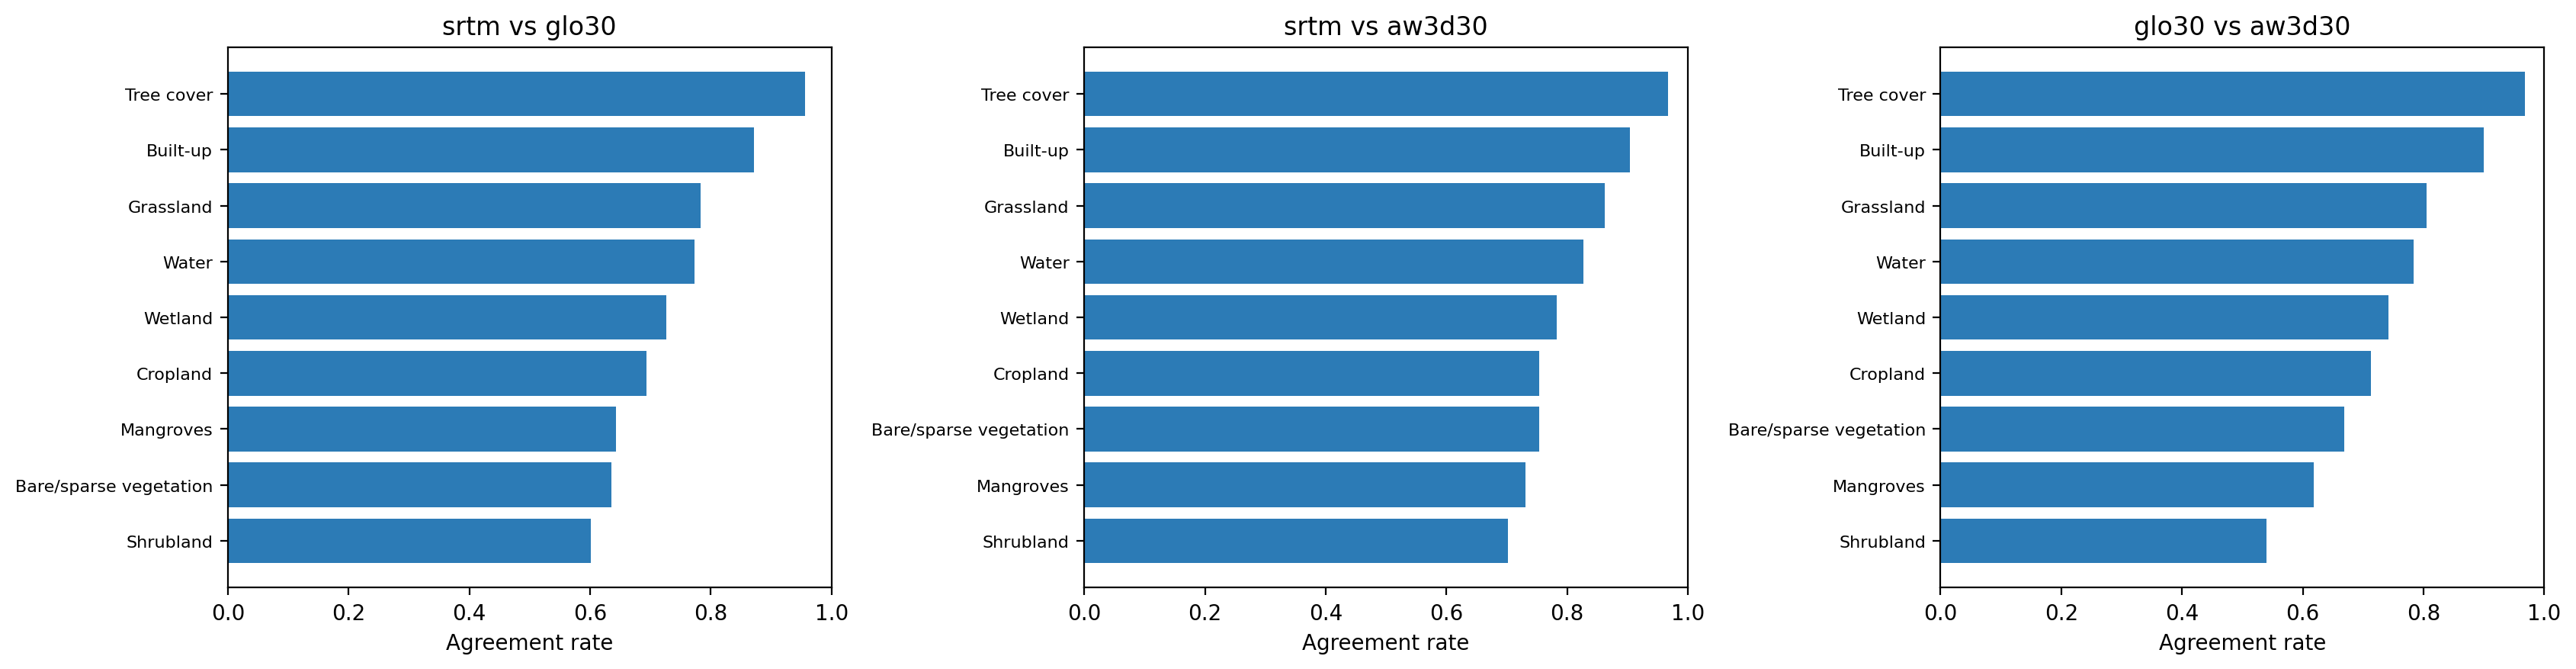
\includegraphics[width=0.95\textwidth]{fig_agreement_v24.png}
\caption{Tingkat kesesuaian kelas (\textit{spatial agreement}) pada masing-masing kelas tutupan lahan ESA WorldCover untuk ketiga pasangan produk elevasi.}
\label{fig:agreement}
\end{figure}

\subsection{Pembahasan}
\label{ssec:pembahasan}

Hasil penelitian ini menjawab keempat rumusan masalah sebagai berikut.
Pertama, dari
aspek karakteristik parameter topografi (Rumusan Masalah~1), SRTM, Copernicus
DEM GLO-30, dan ALOS AW3D30 menghasilkan representasi bentang lahan makro yang
sejalan pada wilayah pesisir Semarang--Demak, namun memiliki perbedaan
sistematis pada elevasi median di dataran rendah pesisir serta variasi
kemiringan lereng lokal akibat perbedaan karakteristik sensor dan datum
vertikal bawaan (EGM96 pada SRTM dibandingkan EGM2008 pada Copernicus DEM
GLO-30 dan ALOS AW3D30). Kedua, dari aspek pemodelan \textit{flood
susceptibility} berbasis Random Forest (Rumusan Masalah~2), ketiga sumber
produk elevasi mampu menghasilkan peta kerawanan banjir dengan daya
diskriminasi yang tinggi, baik pada skema evaluasi \textit{holdout} acak
(ROC-AUC $0{,}932$--$0{,}940$) maupun validasi silang spasial 4-\textit{fold}
(ROC-AUC $0{,}870$--$0{,}890$).

Ketiga, dari aspek sensitivitas performa dan spasial (Rumusan Masalah~3),
\textbf{pergantian sumber produk elevasi terbukti memengaruhi kinerja
prediktif sekaligus mengubah distribusi spasial kelas kerawanan banjir}. Pada
tingkat performa, Copernicus DEM GLO-30 secara konsisten menempati peringkat
tertinggi di atas ALOS AW3D30 dan SRTM pada kelima pengujian \textit{seed}.
Berdasarkan pengujian \textit{block bootstrap}, keunggulan Copernicus DEM
GLO-30 terhadap ALOS AW3D30 ($\Delta\text{AUC}_{\text{GLO-30}-\text{AW3D30}} =
+0{,}0108$ $[+0{,}0041;\,+0{,}0198]$) dan terhadap SRTM
($\Delta\text{AUC}_{\text{SRTM}-\text{GLO-30}} = -0{,}0155$
$[-0{,}0250;\,-0{,}0072]$) bersifat signifikan karena kedua selang kepercayaan
tidak memuat nilai nol, meskipun besaran selisihnya relatif kecil ($\leq
0{,}016$). Sebaliknya, perbedaan performa antara ALOS AW3D30 dan SRTM masih
bersifat marginal karena selang kepercayaannya memuat nilai nol. Pada tingkat
spasial, kesesuaian kelas antarpeta berkisar antara 79,4\% hingga 83,9\%
dengan pergeseran luas kelas ekstrem sekitar 4\% hingga 12\%. Hal ini
menunjukkan bahwa selisih metrik evaluasi yang tampak kecil pada tingkat model
tetap dapat menghasilkan perbedaan delineasi spasial yang bermakna bagi
perencanaan wilayah. Keempat, dari aspek stratifikasi tutupan lahan (Rumusan
Masalah~4), sensitivitas spasial tertinggi terjadi pada tutupan semak belukar
(\textit{shrubland}), lahan terbuka atau vegetasi jarang (\textit{bare/sparse
vegetation}), dan kawasan mangrove (kesesuaian kelas 54,0\%--66,9\%),
sedangkan tutupan pohon dan kawasan terbangun relatif lebih stabil. Temuan ini
sejalan dengan kajian Meadows dkk.\ \cite{meadows2024} serta Tique dkk.\
\cite{Tique2026} yang menunjukkan bahwa variasi galat produk elevasi global
sangat dipengaruhi oleh kondisi tutupan permukaan dan karakteristik morfologi
setempat.

Di luar keempat rumusan masalah utama tersebut, eksperimen ini juga mengungkap
temuan metodologis tambahan mengenai tingginya kepekaan estimasi kinerja model
terhadap \textbf{desain pengambilan sampel kelas non-banjir}. Pergeseran
domain sampel non-banjir dari zona sekitar perairan permanen menuju seluruh
wilayah kajian meningkatkan ROC-AUC validasi silang spasial dari sekitar
$0{,}70$ menjadi $0{,}870$ hingga $0{,}890$ ($\Delta\text{AUC} \approx
0{,}17$), jauh lebih besar daripada selisih antarproduk elevasi
($\Delta\text{AUC} \approx 0{,}01$). Kedua angka ini berasal dari domain
sampel yang berbeda, sehingga perbandingannya bersifat indikatif. Meskipun
\textit{block bootstrap} dan pengujian multi-\textit{seed} mendukung keunggulan
Copernicus DEM GLO-30 pada eksperimen ini, hasil tersebut tidak dimaksudkan
untuk menetapkan satu produk elevasi sebagai pilihan terbaik di seluruh
wilayah atau kejadian banjir lain.

Keterbatasan penelitian ini adalah sebagai berikut. Eksperimen pada penelitian
ini hanya mencakup satu periode kejadian banjir pada satu wilayah kajian
dengan satu nilai \textit{seed} utama untuk pembuatan peta (meskipun
kestabilan metrik telah diuji lintas lima \textit{seed}), serta menggunakan
\textit{flood inventory} berbasis Sentinel-1 sebagai label referensi proksi,
bukan data pengamatan lapangan (\textit{ground truth}) independen.

Terdapat pula perbedaan sifat representasi permukaan
antara SRTM yang berbasis radar pita-C dan Copernicus DEM GLO-30 serta ALOS
AW3D30 yang berkarakteristik \textit{Digital Surface Model} (DSM), ditambah
perbedaan datum vertikal yang dilaporkan tanpa koreksi geoid, granularitas
\textit{block bootstrap} yang masih menggunakan 16 blok kuantil, serta tingkat
kecocokan label sebesar 70\% terhadap sampel penelitian acuan akibat pembaruan
arsip Sentinel-1.

Dari sisi pembentukan label, penyaringan
perairan permanen memakai pita JRC Global Surface Water dengan cakupan
rekaman yang terbatas (masker mencakup sekitar 12,8\%--14,4\% wilayah kajian dan nilai
\textit{occurrence} terbaca pada sekitar 4,3\% wilayah kajian), sehingga label
kejadian banjir hanya dapat terbentuk di dalam area cakupan pita tersebut.
Mengingat batasan tersebut diterapkan secara identik pada ketiga konfigurasi
eksperimen, keadilan perbandingan antarproduk elevasi tetap terjaga; namun,
prediksi kerawanan banjir di luar area cakupan pita tersebut perlu
diinterpretasikan sebagai hasil ekstrapolasi spasial model. Keterbatasan
tersebut menjadi dasar bagi arah pengembangan yang diuraikan pada
Subbab~5.2.

\FloatBarrier

\clearpage

%==================================================================
% BAB V
%==================================================================

\section{Kesimpulan dan Saran}

\subsection{Kesimpulan}

Berdasarkan hasil pemodelan pada Bab~IV, berikut dirangkum jawaban atas
keempat pertanyaan rumusan masalah pada Subbab~1.2:

\begin{enumerate}
\item Karakteristik SRTM, Copernicus DEM GLO-30, dan ALOS AW3D30 terbawa
ke dalam parameter topografi yang dihitung dari masing-masing produk: elevasi,
kemiringan lereng, dan arah lereng berbeda secara statistik dan spasial,
termasuk nilai median elevasi dan offset vertikal antarproduk (Subbab~4.2).
\item Peta probabilitas \textit{flood susceptibility} terbentuk untuk
ketiga sumber elevasi melalui penerapan Random Forest pada prediktor, sampel,
dan konfigurasi model yang identik, sehingga satu-satunya komponen yang
berbeda antarpeta adalah sumber elevasi; pola spasial ketiganya serupa dengan
variasi terbatas pada kelas risiko sangat tinggi (Subbab~4.3 dan Subbab~4.5).
\item Pergantian sumber elevasi menghasilkan perbedaan kinerja yang kecil
tetapi konsisten: keunggulan Copernicus DEM GLO-30 terhadap ALOS AW3D30 dan
terhadap SRTM bersifat konsisten secara statistik pada resampling blok
(Subbab~4.4), sedangkan perbandingan SRTM dan ALOS AW3D30 masih memuat nol
dan bersifat marginal; autokorelasi spasial diperhitungkan melalui validasi
silang spasial dan \textit{bootstrap} pada tingkat blok (Subbab~3.8).
\item Sensitivitas spasial tidak seragam antar kelas tutupan lahan ESA
WorldCover: kelas tutupan pohon paling stabil, diikuti kawasan terbangun,
sedangkan sensitivitas tertinggi terkonsentrasi pada semak belukar, lahan
terbuka atau vegetasi jarang, serta mangrove (Subbab~4.6).
\end{enumerate}

\subsection{Saran}

Berdasarkan hasil dan keterbatasan penelitian, saran yang diajukan adalah
sebagai berikut:

\begin{enumerate}
\item Perluasan cakupan kejadian banjir pada \textit{flood inventory} agar
sensitivitas sumber elevasi dievaluasi pada kondisi banjir yang lebih
representatif.
\item Peningkatan granularitas blok evaluasi spasial (blok lebih banyak dari
16 blok kuantil) untuk mengukur kesensitifan hasil terhadap pilihan skema
blok.
\item Penambahan evaluasi ketidakpastian \textit{flood inventory}, khususnya
terhadap variabilitas arsip Sentinel-1 dan cakupan pita JRC yang telah
dilaporkan sebagai batasan.
\item Penggunaan hasil sensitivitas sebagai bahan pertimbangan pemilihan
produk elevasi terbuka bagi pemetaan kerawanan banjir wilayah pesisir lain
yang menghadapi keterbatasan data topografi beresolusi tinggi.
\end{enumerate}

\FloatBarrier

\clearpage
\printbibliography[title={Daftar Pustaka}]

\end{document}
